\chapter[Diseño de solución]{Diseño de Solución}
\label{cp:design}

\parindent0pt

En la fase de modelado de requerimientos se definieron las bases del sistema, estableciendo sus funcionalidades y características que el prototipo debe cumplir. A partir de estas bases, es posible proceder a la etapa de diseño de solución, que es una transición entre la especificación de lo que el sistema debe hacer y el cómo se construirá, transformando los requerimientos abstractos en una arquitectura concreta y un plan de implementación. El diseño permite obtener una visión integral del sistema antes de iniciar la implementación, lo que facilita la identificación de dependencias e interfaces y asegura que todos los componentes y módulos interactúen de manera coherente. Este proceso de planificación anticipada reduce la probabilidad de encontrar inconsistencias o funcionalidades indefinidas durante las fases de desarrollo y pruebas.

El diseño de la solución, en el marco del modelo en V, se aborda en dos etapas: primero se realiza el diseño de arquitectura y luego el diseño de componentes. Cada una de estas etapas se enfoca en un nivel de abstracción distinto del sistema. El diseño de arquitectura comprende la definición de la estructura general del sistema a través de módulos, mientras que el diseño de componentes se ocupa de los detalles internos de cada módulo.

En la primera etapa, diseño de arquitectura, el sistema se divide en subsistemas o módulos lógicos y se definen sus interacciones, las responsabilidades de cada uno y las tecnologías subyacentes. Este enfoque permite establecer las bases del sistema, abarcando tanto los requerimientos funcionales como los no funcionales. Las decisiones de diseño tomadas en esta etapa se validan posteriormente mediante pruebas de sistema, las cuales se encargan de verificar que todos los módulos trabajen conjuntamente y que el sistema de forma integral satisfaga los requerimientos especificados.

Por otro lado, la segunda etapa es el diseño de componentes, donde se profundiza en los detalles de la arquitectura interna de cada módulo. Esto incluye la especificación de clases, interfaces, flujos de datos y la organización de la lógica de negocio. Los requerimientos funcionales, guiados por las historias de usuario, se traducen en documentos de arquitectura de \gls{software} específicos que posteriormente se implementan en la fase de codificación. Las decisiones de diseño tomadas en esta etapa se verifican a través de las pruebas de integración, que aseguran que los componentes individuales interactúen de forma correcta entre sí.

Los requerimientos funcionales, definidos en el capítulo anterior, son el fundamento para el diseño de la solución y se utilizan en esta etapa a través de las historias de usuario, que guían el diseño de los módulos y componentes. De manera complementaria, los requerimientos no funcionales también se contemplan en la fase de diseño, particularmente en el diseño de arquitectura, donde se establecen las bases para garantizar atributos como la seguridad, el rendimiento y la escalabilidad, incluso si no están directamente asociados a una historia de usuario.

A continuación, se explicará cada una de las etapas del diseño de solución, comenzando con el diseño de arquitectura en la Sección \ref{sec:module-design}, para luego avanzar con el diseño de componentes en la Sección \ref{sec:components-design}.

\section{Diseño de arquitectura}
\label{sec:module-design}

La fase de diseño de arquitectura representa el primer paso en la traducción de los requerimientos del sistema hacia un sistema de \gls{software} funcional. El diseño permite una visión global de la solución, asegurando que todos los componentes y módulos trabajen juntos de manera coherente previo a la implementación. A partir de los requerimientos previamente definidos, se establece un marco de trabajo de alto nivel que estructura la solución en componentes lógicos, delineando sus responsabilidades, las interacciones entre ellos y las tecnologías que los soportan. La salida de esta etapa es la arquitectura del sistema, la cual servirá de base para las decisiones de diseño a un nivel más granular. En el contexto del modelo en V, las decisiones tomadas en esta etapa se validan en la fase de pruebas de sistema, donde se verifica que la arquitectura en su conjunto cumple con las especificaciones definidas en los requerimientos funcionales y no funcionales del sistema.

\begin{figure}[!tb]
    \centering
    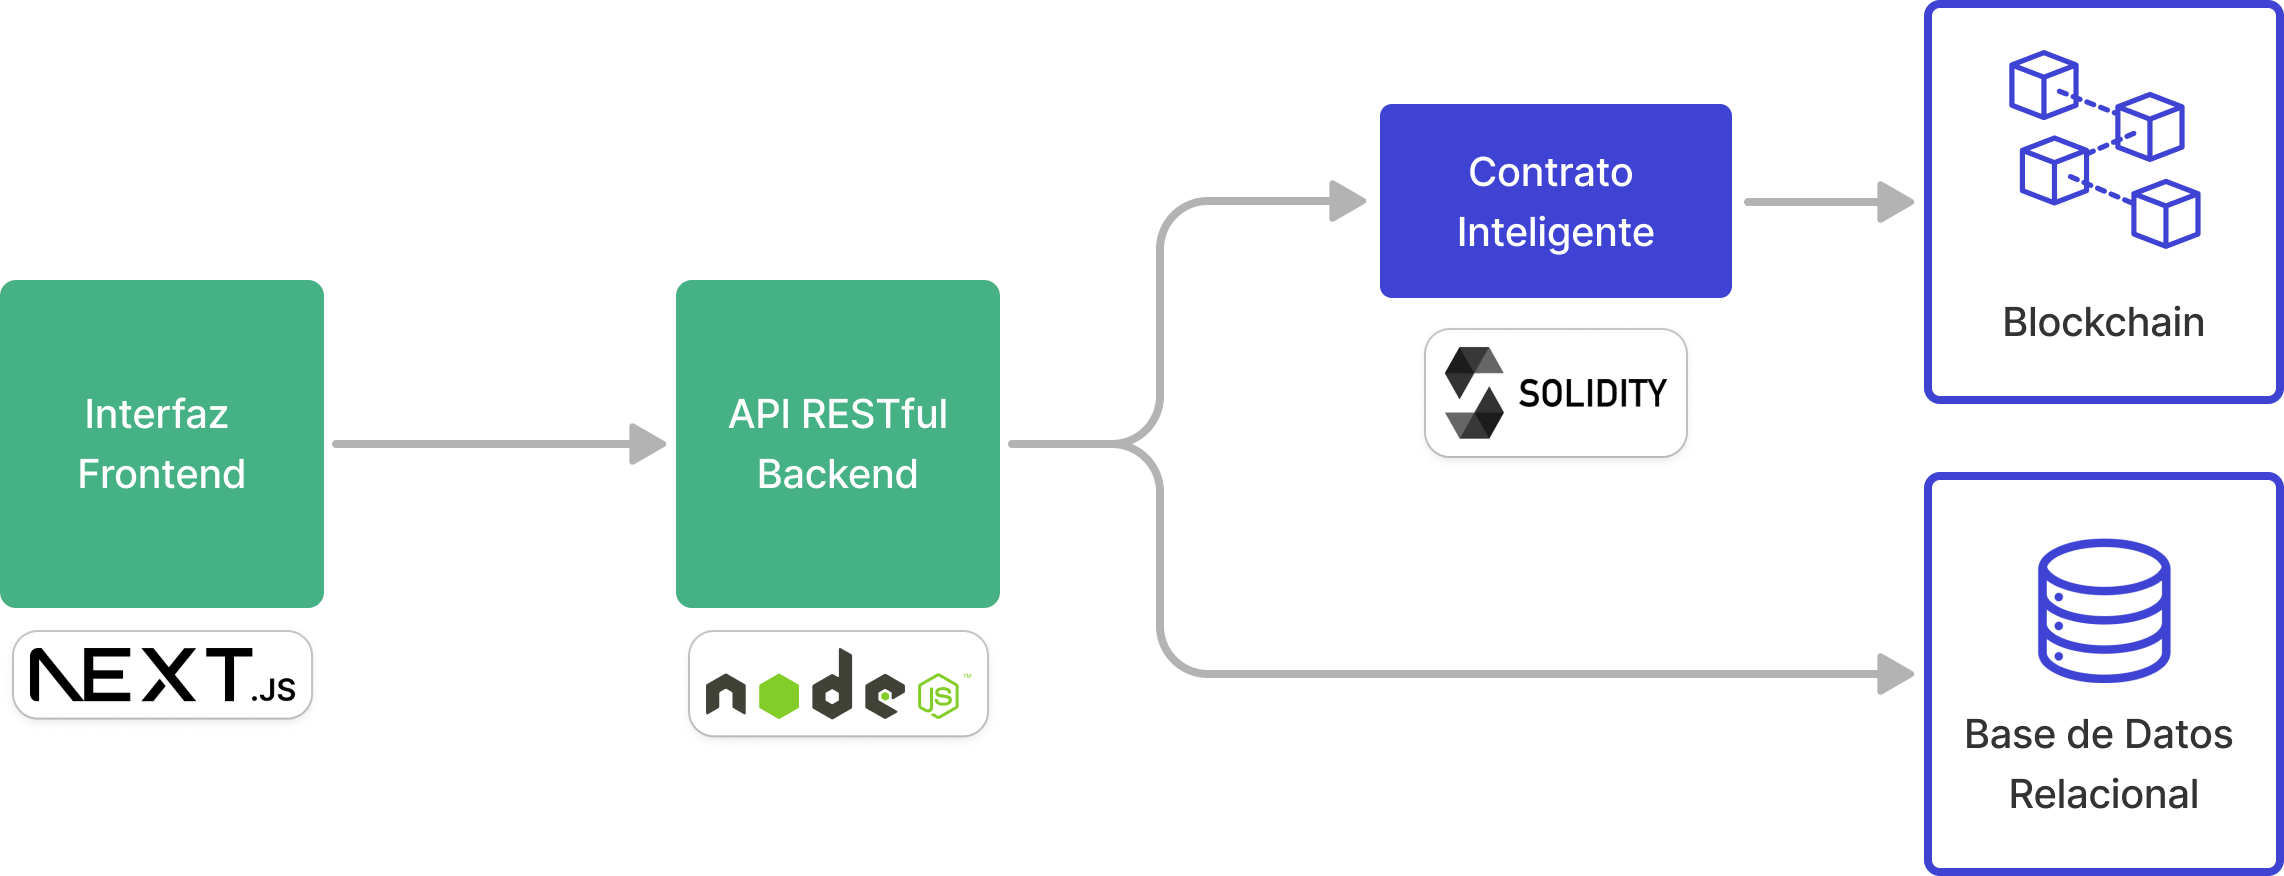
\includegraphics[width=\linewidth]{Figures/software-architecture.png}
    \caption{Arquitectura de módulos del sistema de trazabilidad de envases de vidrio basado en \textit{blockchain}}
    \label{fig:software-architecture}
\end{figure}

Para el prototipo tecnológico de trazabilidad de vidrio basado en \textit{blockchain}, la arquitectura del sistema se concibió siguiendo un enfoque de tres capas lógicas para asegurar una clara separación de responsabilidades y modularidad. Este patrón, común en el desarrollo de aplicaciones web, permite que cada capa se desarrolle, mantenga y escale de forma independiente. En la Figura \ref{fig:software-architecture} se ilustra el diseño de la arquitectura de módulos del sistema elaborado siguiendo este enfoque. La arquitectura se compone de la capa de presentación (\textit{\gls{frontend}}), la capa de lógica de negocio (\textit{\gls{backend}}) y la capa de datos (\textit{\gls{blockchain}} y \gls{basededatos} relacional). La comunicación entre estas capas se define a través de interfaces estandarizadas, lo que promueve una baja dependencia y puede facilitar futuras extensiones e integraciones, por ejemplo, con sistemas de gestión externos o con dispositivos \gls{iot} para automatizar la captura de datos en los procesos productivos.

A su vez, dentro de cada capa del sistema, es necesario definir un criterio para la delimitación de los módulos lógicos dentro de la misma capa. El criterio aplicado en este trabajo se basa en el principio de \textit{cohesión funcional}, el cual plantea agrupar las funcionalidades y responsabilidades del sistema a partir de cada rol de usuario identificado. Siguiendo este criterio, para este trabajo se decidió implementar un módulo específico para cada actor (productor primario, productor secundario, consumidor y centro de reciclaje), así como módulos compartidos para la lógica de negocio transversal, como la autenticación de usuarios o trazabilidad de envases de vidrio. Esta división de responsabilidades reduce el acoplamiento entre los módulos y simplifica el mantenimiento del sistema, en el caso de requerir cambios o actualizaciones en el futuro.

Luego de definir las capas que componen la arquitectura del sistema, es posible proceder a seleccionar las tecnologías más adecuadas para cada uno de los módulos definidos. La elección de tecnologías para cada capa busca satisfacer una serie de criterios técnicos y de negocio, incluyendo la compatibilidad con otras tecnologías, el rendimiento, la escalabilidad y el soporte de la comunidad. El diseño de la arquitectura tecnológica del sistema, incluyendo la definición de tecnologías, se realizó siguiendo un enfoque ``de adentro hacia afuera'', comenzando por la representación de los datos para luego diseñar su acceso (\textit{\gls{backend}}) y finalmente la forma en la cual los datos se muestran (\textit{\gls{frontend}}). Esta perspectiva se elige para priorizar la integridad y la persistencia de la información, que son pilares fundamentales de un sistema basado en \textit{blockchain}. Al abordar primero la capa de datos y la lógica de negocio (es decir, los \glspl{contratointeligente}), se puede garantizar que la estructura central del sistema sea robusta para disminuir el riesgo de inconsistencias en una etapa avanzada de la implementación. Este enfoque, en lugar de uno ``de afuera hacia adentro'' (del \textit{frontend} a los datos), asegura que la lógica de negocio sea el foco principal del diseño, permitiendo que la interfaz de usuario y otras capas de presentación se adapten a la funcionalidad central, y no al revés.

A continuación, se describen las tecnologías seleccionadas, los patrones de diseño aplicados y las decisiones arquitectónicas tomadas para cada capa del sistema. Comenzando por la capa de datos, se explicará la arquitectura desde adentro hacia afuera, siguiendo el flujo de datos desde su representación y almacenamiento hasta la presentación al usuario final.

\subsection{Capa de datos}

La capa de datos constituye el cimiento de todo sistema de software. Se encarga de la persistencia, gestión y recuperación de toda la información del sistema. Las bases de datos relacionales son el tipo de \gls{basededatos} más utilizado actualmente para gestionar información estructurada. Los datos se organizan en tablas, con filas y columnas, y se pueden establecer relaciones entre las distintas tablas mediante claves únicas. Cada columna tiene un nombre y un tipo de dato asociado, mientras que cada fila representa un registro único dentro de la tabla y su contenido debe cumplir con el tipo de dato definido para cada columna. Por ejemplo, se podría definir una tabla ``Usuario'', para almacenar información sobre los usuarios del sistema, incluyendo columnas como ``nombre'' de tipo texto, ``correo electrónico'' de tipo texto y ``fecha de registro'' de tipo fecha, entre otras columnas. Cada fila en esta tabla representaría un usuario específico, con su nombre, correo electrónico y la fecha en que se registró en el sistema, entre otros datos. Las principales ventajas de las bases de datos relacionales radican en su capacidad para garantizar la uniformidad de los datos a través de esquemas definidos para cada tabla, así como la facilidad para realizar consultas y análisis complejos de manera eficiente. Sin embargo, su naturaleza centralizada las hace susceptibles a manipulaciones manuales difíciles de detectar, lo que justifica la necesidad de una tecnología complementaria, como la \textit{blockchain}, para registrar información que requiere garantías de integridad.

En este prototipo, la tecnología \textit{blockchain} resulta apropiada para registrar la información clave del sistema, que requiere inmutabilidad y transparencia para fomentar la confianza entre los distintos actores. Ejemplos de este tipo de información pueden ser la propiedad de los lotes de envases de vidrio o la \gls{trazabilidad} de los envases reciclados. Por este motivo, se tomó la decisión estratégica de combinar la \textit{blockchain} con una \gls{basededatos} relacional con el objetivo de resolver la necesidad de equilibrio entre la seguridad y la transparencia, con el rendimiento y la escalabilidad. La \textit{blockchain}, por su naturaleza, provee una fuente de información segura y transparente, pero puede presentar limitaciones en cuanto a la velocidad de las transacciones y el volumen de datos que permite consultar eficientemente. Para abordar estas limitaciones, es que se decidió utilizar la \textit{blockchain} como base de datos principal del sistema, mientras que se decidió utilizar una base de datos relacional complementaria para almacenar datos auxiliares e indexar los datos de acceso frecuente, como los perfiles de usuario, los metadatos de los lotes (\textit{id}, propietario, estado, etc.) y otros datos de soporte que no requieren inmutabilidad. La relación entre ambas fuentes de datos se maneja mediante identificadores únicos que se almacenan en la \textit{blockchain}, sirviendo como una referencia a los datos detallados en la base de datos relacional. La capa \textit{\gls{backend}} es responsable de mantener la consistencia entre ambas fuentes de información (\textit{blockchain} y base de datos relacional) a la hora de persistir nueva información o actualizar información existente. Este enfoque híbrido permite proveer una recuperación de información ágil y una experiencia de usuario fluida sin poner en compromiso la integridad de los datos sensibles.

Luego de definir la estrategia de almacenamiento y gestión de datos, es posible proceder a seleccionar las tecnologías específicas que se utilizarán, tanto para la base de datos relacional como para la plataforma \textit{blockchain}, ya que existen múltiples opciones en el mercado.

En el caso de la base de datos relacional, se optó por el uso de MariaDB\footnote{\url{https://mariadb.org/documentation/}}, una base de datos de código abierto elegida por su sencillez y familiaridad, ya que el uso que se le dará en este trabajo es complementario y no hace falta utilizar una alternativa más compleja. MariaDB cuenta con un amplio soporte, librerías y documentación disponible para conectarse a ella de forma estandarizada desde cualquier lenguaje o \textit{framework} utilizado en la capa \textit{backend}.

Por otro lado, para la tecnología \textit{blockchain}, la elección de una plataforma adecuada puede determinar la complejidad y tiempo de implementación del sistema.  La tecnología \textit{blockchain} no se implementa desde cero, sino que se utilizan plataformas ya desarrolladas y probadas que ofrecen características y funcionalidades específicas. Estas plataformas, conocidas como protocolos \textit{blockchain}, varían en aspectos como su \gls{mecanismodeconsenso}, lenguaje de programación y comunidad de desarrolladores. Para este trabajo, se analizaron cinco de las plataformas líderes en la industria para su análisis y comparación: Hyperledger Fabric, Ethereum, Polkadot, VeChain y Cardano. Estas plataformas se seleccionaron por su relevancia y características técnicas, evaluando su idoneidad para el caso de uso específico de trazabilidad en la \gls{cadenadesuministro} del vidrio.

\textbf{Hyperledger Fabric}\footnote{\url{https://hlf.readthedocs.io/en/latest/}}
es una plataforma de código abierto diseñada para uso empresarial, que forma parte de la Fundación Linux \cite{androulaki2018hyperledger}. Se caracteriza por su arquitectura modular y configurable, ideal para una amplia gama de casos de uso en la industria. A diferencia de las redes públicas, es una plataforma permisionada, lo que significa que los participantes se conocen y confían entre sí. Admite \glspl{contratointeligente} en lenguajes de programación comunes como Java\footnote{\url{https://www.java.com/en/}} y Node.js\footnote{\url{https://nodejs.org/en}}, lo que reduce la curva de aprendizaje. Hyperledger no requiere una \gls{criptomoneda} nativa, lo que elimina ciertos riesgos de ataque y permite que la plataforma se implemente con costos operativos similares a los de cualquier otro sistema distribuido.

\textbf{Ethereum}\footnote{\url{https://ethereum.org/en/developers/docs/}}
es una plataforma de código abierto y pública que permite a los desarrolladores crear contratos inteligentes y aplicaciones descentralizadas (\gls{dapps}). Se considera una computadora mundial descentralizada, alimentada por su \gls{criptomoneda} nativa, Ether. Ethereum fue pionera en la creación de contratos inteligentes y ha mantenido un liderazgo en la industria desde su lanzamiento en 2015. Los contratos se escriben en Solidity\footnote{\url{https://www.soliditylang.org/}}, un lenguaje de programación de dominio específico que se ejecuta en la red de Ethereum. Este lenguaje de programación en la actualidad es el más utilizado para el desarrollo de contratos inteligentes. Aunque Ethereum se lanzó con un protocolo de consenso de Prueba de Trabajo (\acrshort{pow}), la plataforma ha migrado a la Prueba de Participación (\acrshort{pos}) para mejorar su eficiencia energética y escalabilidad.

\textbf{Polkadot}\footnote{\url{https://docs.polkadot.com/}}
es una plataforma de código abierto que busca facilitar la interoperabilidad entre diferentes \textit{blockchains}. Su objetivo es crear una red escalable y segura que pueda soportar una amplia gama de aplicaciones descentralizadas. Su arquitectura se basa en una cadena principal (\textit{relay chain}) y múltiples cadenas que se conectan a ella (\textit{parachains}), permitiendo que las \textit{blockchains} se comuniquen entre sí de manera eficiente a través de la \textit{relay chain}. Utiliza un protocolo de consenso derivado de \acrshort{pos}, llamado Prueba de Participación Nominada (\acrshort{npos}, \textit{\acrlong{npos}}) y su \gls{criptomoneda} nativa es DOT. Las aplicaciones se desarrollan con Substrate\footnote{\url{https://polkadot.com/platform/sdk/}}, un \textit{framework} modular escrito en Rust\footnote{\url{https://rust-lang.org/}}, que también es compatible con contratos inteligentes escritos en Solidity.

\textbf{VeChain}\footnote{\url{https://docs.vechain.org/}}
es una plataforma de código abierto dedicada específicamente a la trazabilidad y la autenticación de productos en la \gls{cadenadesuministro}. Combina tecnología \textit{blockchain} con \gls{rfid} e \gls{iot} para rastrear productos desde la producción hasta el consumidor final. Es una plataforma permisionada, donde los participantes se conocen y confían mutuamente, lo que permite una mayor privacidad y confidencialidad. Utiliza una arquitectura de dos \textit{\glspl{token}} (VET y VTHO) y un protocolo de consenso de Prueba de Autoridad (\acrshort{poa}). Al ser compatible con Solidity, facilita la migración de aplicaciones existentes de Ethereum.

\textbf{Cardano}\footnote{\url{https://docs.cardano.org/}}
es una plataforma de \textit{blockchain} de código abierto que se enfoca en la creación de una red escalable, segura y sostenible. Se distingue por su enfoque científico y riguroso, utilizando evidencia formal y revisión por pares para garantizar la seguridad y confiabilidad de la plataforma. Para programar aplicaciones se utiliza el lenguaje de programación funcional Haskell, que permite la verificación formal de los contratos inteligentes. También se pueden desarrollar contratos utilizando Plutus\footnote{\url{https://docs.cardano.org/developer-resources/smart-contracts/plutus}}, un lenguaje de dominio específico basado en Haskell\footnote{\url{https://www.haskell.org/}}. La red utiliza un protocolo de consenso \acrshort{pos} y su \gls{criptomoneda} nativa es ADA.

En la Tabla \ref{tab:blockchain-comparison}, se presenta un resumen comparativo de los protocolos \textit{blockchain} analizados, destacando los aspectos relevantes de cada uno para la selección del más adecuado para este trabajo.


\begin{xltabular}{\textwidth}{@{} Y C{3cm} C{2cm} C{3cm} C{2cm} C{2cm} @{}}
    \caption{Comparación de plataformas \textit{blockchain}}
    \label{tab:blockchain-comparison} \\
	\toprule
	\textbf{Tecnología} & \textbf{Hyperledger} & \textbf{Ethereum} & \textbf{Polkadot} & \textbf{VeChain} & \textbf{Cardano} \\
	\midrule
\endfirsthead

\toprule
\textbf{Tecnología} & \textbf{Hyperledger} & \textbf{Ethereum} & \textbf{Polkadot} & \textbf{VeChain} & \textbf{Cardano} \\
\endhead

\multicolumn{6}{r}{\footnotesize Continúa en la siguiente página}
\\\bottomrule
\endfoot

\bottomrule
\endlastfoot

    Consenso & Flexible & \acrshort{pow} - \acrshort{pos} & \acrshort{npos} & \acrshort{poa} & \acrshort{pos} \\ 
    \hline
    Lenguaje & Java, Go, Node.js & Solidity & Rust, Solidity & Solidity & Haskell \\ 
    \hline
    Interoperabilidad & Limitada & Limitada & Alta & Limitada & Limitada \\ 
    \hline
    Adopción & Alta & Muy alta & Media & Media & Media \\ 
    \hline
    Comunidad & Grande & Grande & Grande & Mediana & Grande \\ 

\end{xltabular}

Luego de realizar el análisis comparativo entre protocolos \textit{blockchain}, se llega a la determinación de que Ethereum resulta ser la tecnología más adecuada para este trabajo por múltiples razones. En primer lugar, su naturaleza pública está alineada con el objetivo del proyecto, ya que permite a cualquier persona unirse a la red y verificar el estado de la cadena de forma transparente, sin necesidad de permisos, como puede ocurrir en las plataformas permisionadas como Hyperledger. A su vez, otro factor influyente en esta elección es la adopción del \gls{mecanismodeconsenso} \acrshort{pos} en la red Ethereum, que es más eficiente energéticamente que \acrshort{pow}, de modo que se alinea directamente con los objetivos de \gls{sostenibilidad} ambiental del proyecto. Además, Ethereum posee la mayor comunidad de desarrolladores entre las plataformas analizadas y una alta adopción en la industria, lo que garantiza un soporte continuo y una amplia gama de herramientas y recursos a su disposición. Su lenguaje de programación, Solidity, es de alto nivel y fácil de aprender en comparación a lenguajes como Rust y Haskell, permitiendo la creación de aplicaciones complejas de manera eficiente. Finalmente, existe una amplia variedad de herramientas que permiten conectar otras tecnologías y sistemas con Ethereum, facilitando la integración con la base de datos relacional y la capa \textit{backend} del sistema.

\begin{figure}[!tb]
    \centering
    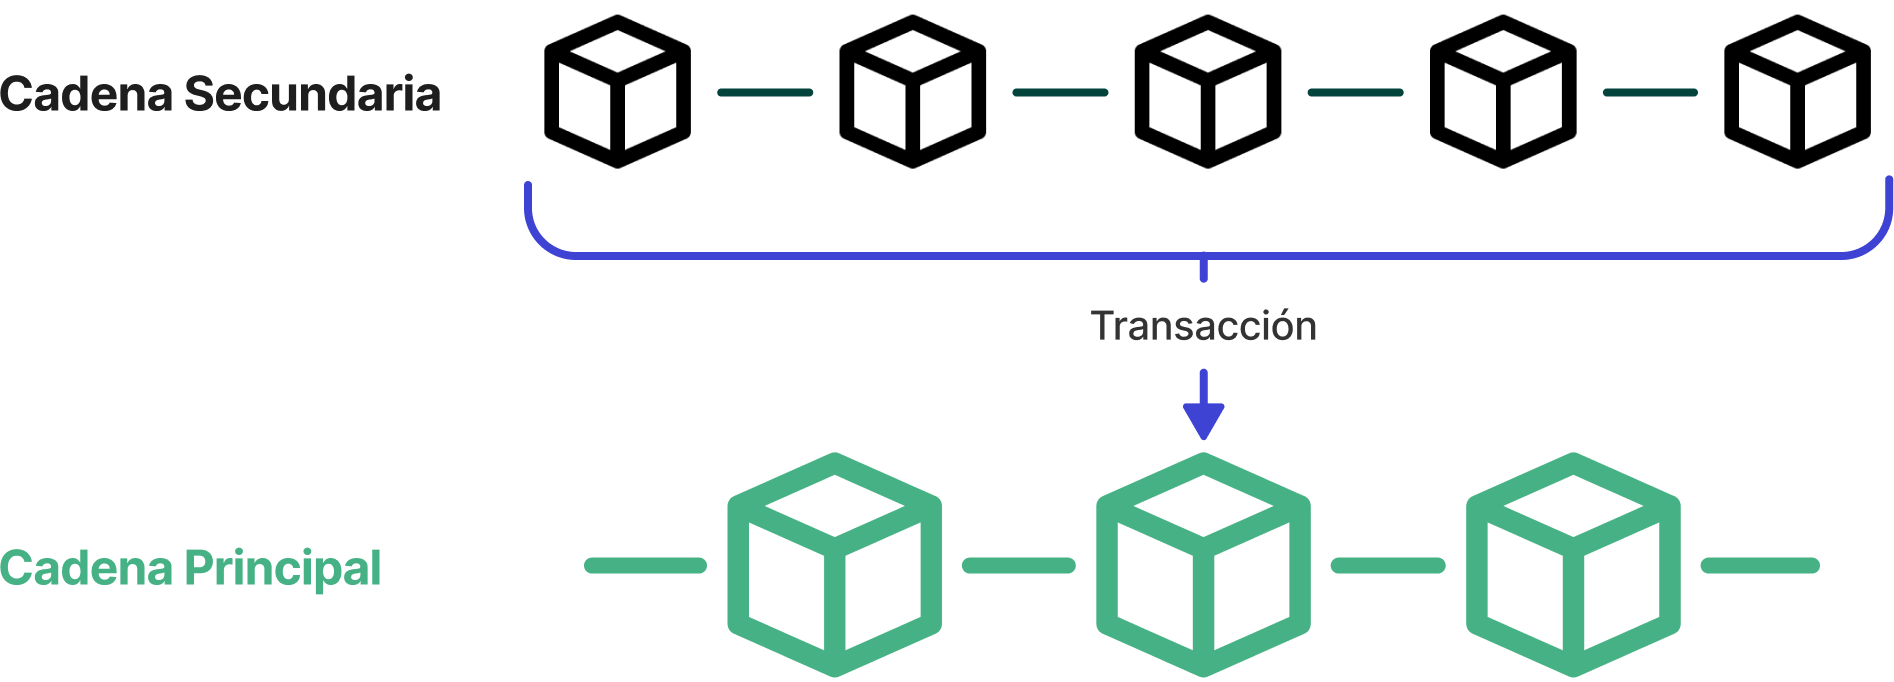
\includegraphics[width=0.9\linewidth]{Figures/blockchain-layer-2.png}
    \caption{Funcionamiento de una cadena secundaria sobre Ethereum}
    \label{fig:ethereum-layer-2}
\end{figure}

Sin embargo, Ethereum presenta algunas desventajas, como los altos costos de transacción y alta latencia de red, que pueden afectar la experiencia del usuario y la viabilidad económica del sistema. Afortunadamente, en la actualidad existen múltiples soluciones para mitigar estos problemas. En particular, para mitigar los altos costos y la latencia de la red de Ethereum para esta aplicación de trazabilidad que puede alcanzar un volumen de datos considerable, se decidió realizar el despliegue de los contratos en una cadena secundaria de Ethereum, que permite procesar las transacciones en una cadena complementaria de alto rendimiento y bajo costo para luego sincronizarla con la cadena principal mediante una única transacción (Figura \ref{fig:ethereum-layer-2}), lo que reduce costos y aumenta la escalabilidad, sin comprometer la seguridad ni la integridad de los datos de la \textit{blockchain} Ethereum. A su vez, se eligió hacer uso del \textit{framework} Hardhat\footnote{\url{https://hardhat.org}} para el desarrollo y despliegue de los \glspl{contratointeligente}, ya que es una herramienta ampliamente adoptada que facilita la implementación y ejecución de pruebas unitarias y de integración sobre contratos inteligentes en Solidity.

\subsection{Capa backend}

La capa de lógica de negocio, generalmente conocida como \textit{\gls{backend}} o \gls{api} (\textit{Application Programming Interface}), actúa como el cerebro del sistema. Su propósito principal es implementar y ejecutar las reglas de negocio del sistema, orquestar la interacción entre las distintas capas (capa \textit{frontend} y capa de datos), y exponer una interfaz estandarizada a través de la cual otros componentes puedan interactuar con la funcionalidad del sistema, sin depender de su implementación interna.

Para este prototipo, se ha optado por implementar una arquitectura desacoplada, donde la capa de presentación (\textit{frontend}) y la capa de lógica de negocio se desarrollan de forma independiente. Este tipo de arquitectura desacoplada resulta necesaria para un sistema de las características de este trabajo. A diferencia de una arquitectura monolítica, este enfoque promueve la modularidad y la escalabilidad, permitiendo que la interfaz de usuario pueda evolucionar o ser reemplazada sin afectar la lógica de negocio central de la aplicación. Este diseño responde directamente al requerimiento no funcional de interoperabilidad (RNF-05), ya que la \gls{api} de trazabilidad está pensada para ser el punto de integración principal no solo para el \textit{frontend} del prototipo, sino también para sistemas de gestión preexistentes, dispositivos \gls{iot} y otras aplicaciones de terceros que pudieran surgir en el futuro para la \gls{trazabilidad} de procesos de la \gls{cadenadesuministro} y reciclaje de los envases de vidrio.

Para la implementación de la capa \textit{backend} se tomó la decisión de utilizar la tecnología Node.js\footnote{\url{https://nodejs.org/es}}, un entorno de ejecución del lenguaje JavaScript\footnote{\url{https://developer.mozilla.org/es/docs/Web/JavaScript}} que permite crear servidores, aplicaciones web, herramientas de línea de comandos y \textit{scripts}. A su vez, JavaScript es un lenguaje de programación de alto nivel, interpretado y dinámico, que es ampliamente conocido y utilizado para el desarrollo web tanto en \textit{frontend} como en \textit{backend}. Su curva de aprendizaje es relativamente baja y es el lenguaje que se utiliza para dar dinamismo a las páginas web. Sin embargo, su uso también se ha extendido al lado del servidor gracias a entornos de ejecución como Node.js, lo que ha permitido a los desarrolladores crear aplicaciones web completas utilizando un único lenguaje de programación. Su popularidad y amplia adopción en la industria, se deben a su flexibilidad y a la gran cantidad de librerías y \textit{frameworks} que se han desarrollado para este lenguaje, que permiten construir tanto aplicaciones web simples, como sistemas complejos y escalables.

Existen múltiples motivos que justifican la elección del entorno Node.js para el desarrollo de la capa \textit{backend} de este trabajo. En primer lugar, considerando el alcance limitado del trabajo, JavaScript resulta ser un lenguaje propicio debido a su baja curva de aprendizaje y su flexibilidad para ser utilizado tanto en la capa \textit{backend} como en la capa \textit{frontend}, lo que facilita el proceso de desarrollo al permitir que el mismo desarrollador trabaje en ambas capas sin necesidad de cambiar de lenguaje. Existen múltiples lenguajes y \textit{frameworks} ampliamente utilizados en la industria para desarrollar la capa \textit{backend} de aplicaciones web, como Java con Spring Boot, Python con Django o Flask y Ruby on Rails, pero la posibilidad de utilizar el mismo lenguaje tanto en \textit{frontend} como en \textit{backend}, simplifica el proceso de desarrollo en equipos pequeños o unipersonales y ayuda a facilitar el mantenimiento del código en el futuro. A su vez, Node.js ofrece un excelente soporte para la interacción con la red de Ethereum, mediante una serie de librerías ampliamente adoptadas y probadas en la comunidad, como pueden ser Ethers.js y Web3.js. Por último, la amplia adopción de Node.js en la industria y la disponibilidad de herramientas para pruebas unitarias facilitan el desarrollo y el mantenimiento del sistema. 

\begin{figure}[!tb]
    \centering
    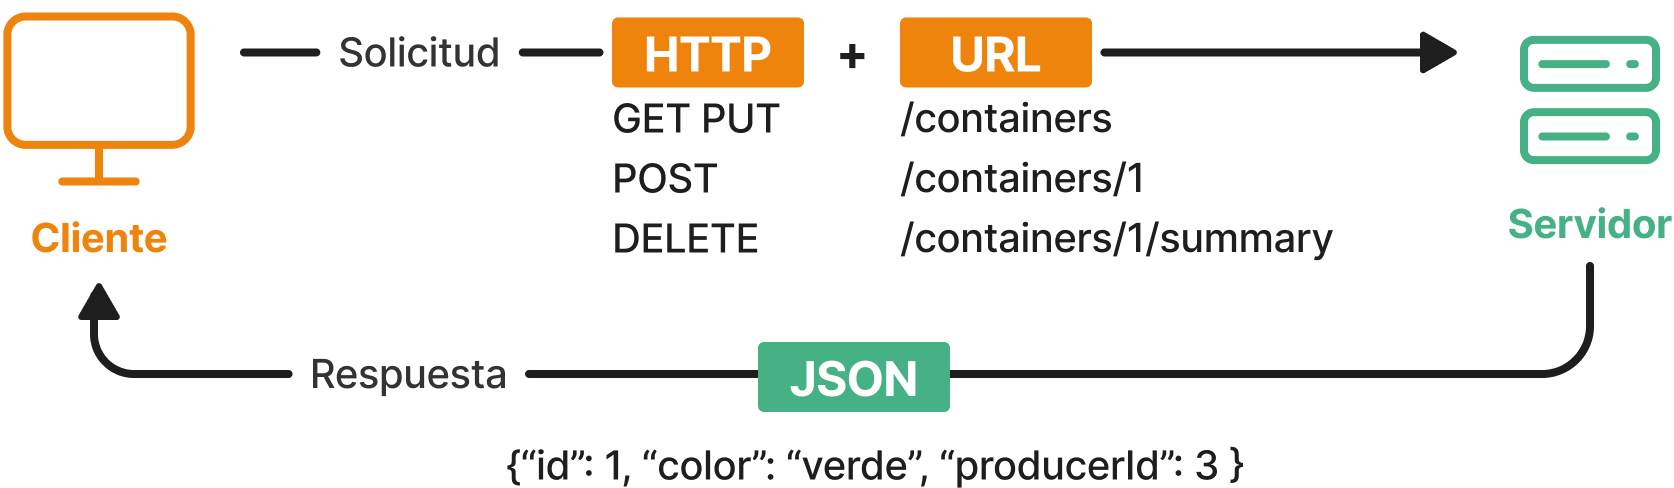
\includegraphics[width=\linewidth]{Figures/backend-api-rest.png}
    \caption{Funcionamiento de una API REST}
    \label{fig:api-rest}
\end{figure}

Por otro lado, la comunicación del \textit{backend} con las demás capas del sistema debe implementarse a través de interfaces bien definidas. La \gls{api} \textit{backend} implementa el estándar \textit{\gls{apirest}} para la comunicación con la capa de presentación. El estándar \acrshort{rest} (\textit{\acrlong{rest}}), ilustrado en la Figura \ref{fig:api-rest}, define una arquitectura para la comunicación entre sistemas que se basa en el uso del protocolo \gls{http} para intercambiar información sin mantener un estado entre intercambios. Una \gls{apirest} utiliza los métodos estándar de \gls{http} (como \textit{GET}, \textit{POST}, \textit{PUT} y \textit{DELETE}) para realizar operaciones sobre los recursos del sistema y adopta el formato \gls{json} para el intercambio de datos. La \gls{api} se estructura en un conjunto de \textit{\glspl{endpoint}}, cada uno representando una acción sobre un recurso específico del sistema, ya sea crear, leer, actualizar o eliminar el recurso. Por ejemplo, el \textit{frontend} del sistema podría enviar una solicitud \textit{GET} al \textit{endpoint} ``/api/containers'' para solicitar la lista de envases de vidrio producidos por cierto productor primario. En este caso, el \textit{backend} respondería con la información solicitada en formato \gls{json} y el \textit{frontend} podría utilizar esta información para actualizar la interfaz de usuario, mostrando el listado de los envases de vidrio correspondientes al usuario.

Dentro del entorno de Node.js, existen múltiples librerías y \textit{frameworks} que facilitan el desarrollo de \glspl{apirest}. La opción más popular y ampliamente adoptada es Express.js\footnote{\url{https://expressjs.com/}}, un \textit{framework} minimalista y flexible que proporciona las utilidades esenciales para la construcción de \glspl{apirest}. Entre sus principales ventajas se encuentran su simplicidad, flexibilidad y extensibilidad. Gracias a estas características, Express.js es utilizado para construir \gls{apirest} directamente, pero también ha sido utilizado como base de múltiples \textit{frameworks} de desarrollo de \glspl{apirest} más complejos, como Nest.js y Sails.js, entre otros. Estos \textit{frameworks} extienden las funcionalidades de Express.js y facilitan el desarrollo de \glspl{api} en Node.js, añadiendo funcionalidades adicionales que mejoran la mantenibilidad y escalabilidad de las \glspl{apirest}. Sin embargo, estos \textit{frameworks} suelen imponer una estructura más rígida y una curva de aprendizaje más pronunciada que Express.js. Por este motivo, se decidió utilizar Express.js como base para el desarrollo de la \gls{api} del sistema, ya que no impone restricciones adicionales sobre el modelo arquitectónico y permite una implementación eficiente y escalable, sin sacrificar la flexibilidad necesaria para adaptarse a los requerimientos específicos del sistema.

Finalmente, para la interacción con la capa de datos, el \textit{backend} se conecta a la base de datos relacional mediante librerías de conexión estandarizadas y a la \textit{blockchain} a través de librerías de interacción con \glspl{contratointeligente}, lo que permite un acceso unificado a los datos, abstrayendo la complejidad de cada fuente de datos y proporcionando una interfaz coherente para la capa \textit{frontend} del sistema.

\subsection{Capa frontend}

La capa de presentación, conocida habitualmente como \textit{\gls{frontend}}, es la interfaz de usuario web que permite a los distintos actores de la cadena de suministro interactuar con el sistema de trazabilidad del vidrio. Su objetivo es traducir la lógica de negocio y los datos que provienen de la API en una experiencia visual y funcional, permitiendo que los usuarios interactúen con el prototipo de manera intuitiva. El \textit{frontend} es la cara visible del sistema completo.

Para este prototipo, se tomó la decisión de implementar de forma desacoplada la interfaz de la lógica de negocio, con el objetivo de reforzar la mantenibilidad y flexibilidad del sistema. Esta separación es propicia para que la interfaz de usuario pueda evolucionar de manera independiente de la lógica, adaptándose a nuevas necesidades, experiencias de usuario o tecnologías sin afectar el funcionamiento del sistema. Con este esquema, es factible que en un futuro, cada actor de la cadena tenga acceso a una interfaz a medida de sus necesidades. Por ejemplo, para un productor de envases de vidrio, se podría desarrollar una aplicación de escritorio con métricas de negocio sobre su producción y venta, mientras que para los consumidores, se podría crear una aplicación móvil que muestre puntos de reciclaje y ofrezca incentivos por reciclar. Aunque el prototipo desarrollado para este trabajo final presenta una interfaz web unificada para todos los actores, el diseño modular facilita la creación de estas aplicaciones independientes en el futuro.

La elección tecnológica para esta capa estuvo focalizada en encontrar \textit{frameworks} y librerías que promuevan la modularidad y la eficiencia durante el desarrollo. En primer lugar, se determinó utilizar React\footnote{\url{https://es.react.dev/}} como librería base para la construcción de la interfaz, debido a su modelo de desarrollo basado en componentes, que promueve la reutilización de código. A su vez, para potenciar React, se optó por hacer uso del \textit{framework} Next.js\footnote{\url{https://nextjs.org/docs}}, que agrega funcionalidades extra a React para facilitar aún más el desarrollo de aplicaciones web modulares y de alto rendimiento, combinando técnicas como generación de sitios estáticos y renderizado en el servidor. Por otro lado, para el diseño de las interfaces web se utiliza el lenguaje de estilado \gls{css}\footnote{\url{https://developer.mozilla.org/en-US/docs/Web/CSS}}, que en este prototipo se complementó con el uso de la librería Tailwind \gls{css}\footnote{\url{https://tailwindcss.com/}} que promueve una estética moderna y una sintaxis simplificada dentro del código.

La comunicación del \textit{frontend} con el \textit{\gls{backend}} se realiza exclusivamente a través de llamadas a la \gls{apirest}. La interfaz no contiene la lógica de negocio, sino que actúa como un cliente ligero que envía datos al \textit{backend} (por ejemplo, al registrar un nuevo lote) y recibe la respuesta, la cual es luego presentada al usuario. Este modelo garantiza que el \textit{frontend} se enfoque en la interacción y la visualización, mientras la lógica crítica reside en el \textit{backend}. Debido a que el \textit{frontend} se enfoca únicamente en la visualización de información, es necesario implementar un sistema de autenticación y autorización unificado entre \textit{frontend} y \textit{backend} que permita a cada usuario visualizar e interactuar únicamente con las funcionalidades propias de su rol. Por este motivo, para gestionar la autenticación de usuarios en este proyecto, se determinó hacer uso del servicio Firebase Authentication\footnote{\url{https://firebase.google.com/docs/auth}}, que gestiona la autenticación de usuarios e implementa de forma abstracta el estándar de autorización OAuth 2.0\footnote{\url{https://oauth.net/2/}}, asegurando que solo los actores con los permisos adecuados puedan acceder a cada recurso del sistema.

\begin{figure}[!t]
    \centering
    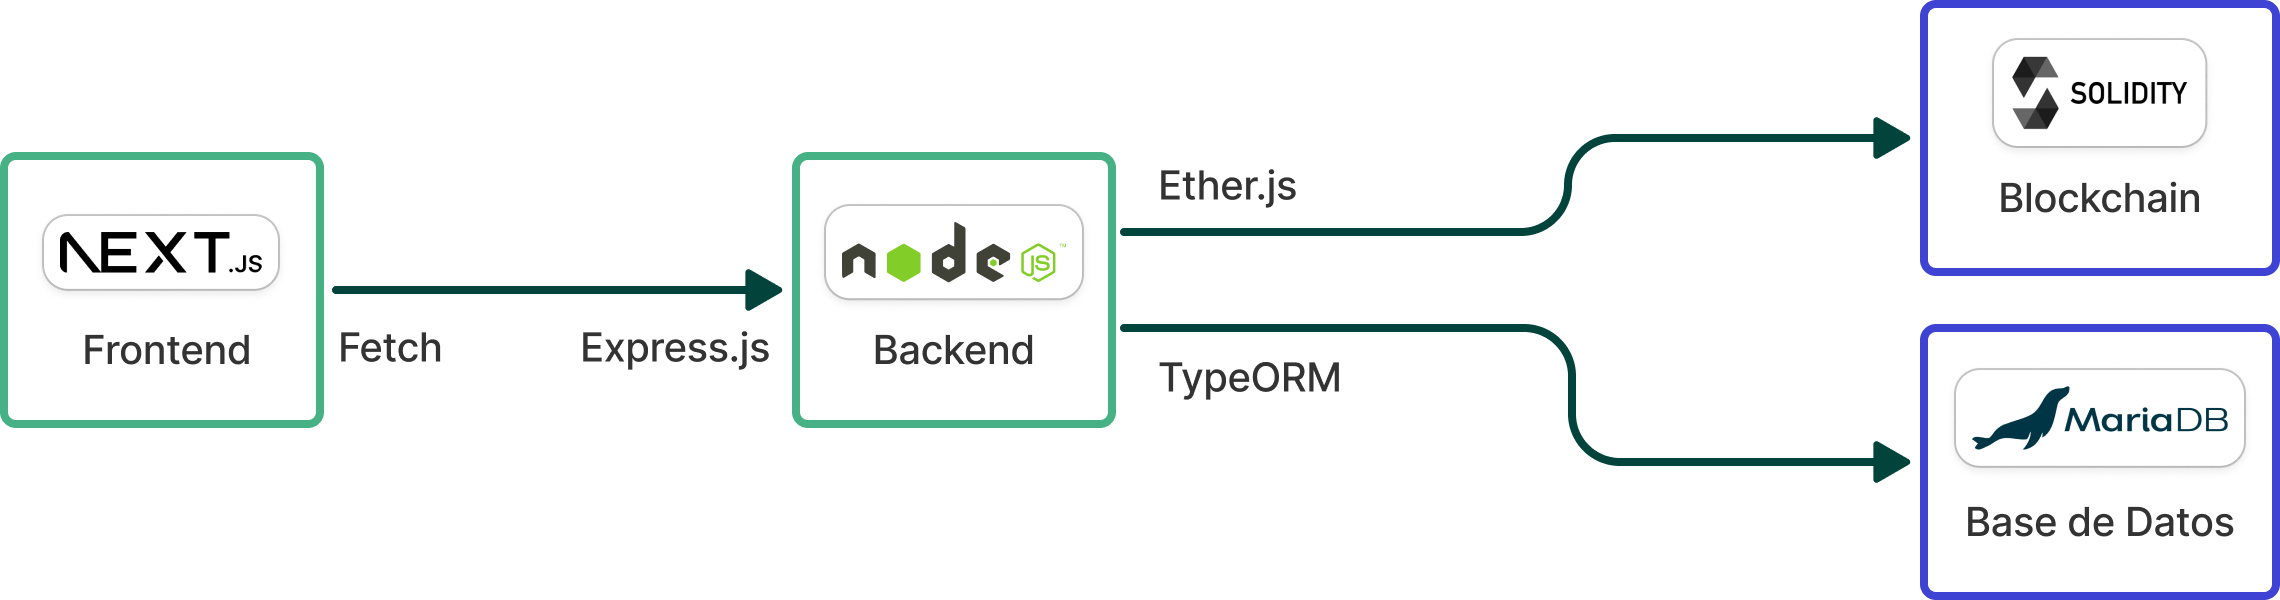
\includegraphics[width=\linewidth]{Figures/system-architecture.png}
    \caption{Arquitectura del sistema con librerías elegidas para comunicación entre módulos}
    \label{fig:system-architecture}
\end{figure}

Por último, en la Figura \ref{fig:system-architecture} se puede observar la arquitectura general del sistema, donde Next.js se utiliza para el desarrollo del \textit{frontend}, que se comunica con el \textit{backend}, que se implementa en Node.js y utiliza el \textit{framework} Express.js para recibir las solicitudes, mientras que emplea librerías específicas para comunicarse con los contratos inteligentes en Solidity y con la base de datos relacional de MariaDB. 
Luego de definir la arquitectura de la aplicación web, incluyendo la definición de capas, la comunicación entre ellas y los lenguajes de programación a utilizarse, es posible comenzar con la etapa de diseño de componentes. En esta segunda etapa de diseño, se define la arquitectura interna de cada capa o módulo definido en la etapa anterior. En la próxima sección, se detallará el diseño de componentes de este sistema, que abarca la estructura interna del \textit{frontend}, la API y la capa de datos.

\section{Diseño de componentes}
\label{sec:components-design}

La segunda etapa de diseño, el diseño de componentes, tiene como objetivo detallar la arquitectura interna de los módulos definidos en la fase anterior. Su propósito es traducir la arquitectura de alto nivel en un plan de construcción específico, que incluye la estructura de la interfaz de usuario, la arquitectura de la API y el modelo de datos. Esta fase toma como punto de partida los requerimientos del sistema y la arquitectura de módulos previamente definida, y su resultado es un conjunto de especificaciones detalladas que guiarán la implementación de cada módulo del software. De esta forma, se busca asegurar la cohesión interna de cada módulo y su correcta interacción con los demás. A su vez, cada decisión de diseño tomada en esta etapa se verificará posteriormente en la fase de pruebas de integración, que valida la correcta comunicación entre los componentes del sistema.

A continuación, se presentarán las decisiones de diseño tomadas para cada uno de los módulos definidos en la arquitectura del sistema: la capa de datos, la capa de lógica de negocio (\textit{backend}) y la capa de presentación (\textit{frontend}).

\subsection{Arquitectura de datos}

El diseño de la arquitectura de datos representa un componente central de este trabajo, ya que debe integrar de manera transparente y eficiente la naturaleza descentralizada de la \textit{blockchain} con la eficiencia y escalabilidad de una \gls{basededatos} relacional para cumplir con los requerimientos no funcionales del sistema (RNF-01: Transparencia, RNF-03: Escalabilidad y RNF-06: Integridad). La solución definida durante la etapa de diseño de arquitectura propone un modelo de datos híbrido para optimizar el almacenamiento y la recuperación de información. En este esquema, la \textit{blockchain} se utiliza como una capa de confianza inmutable, mientras que la base de datos relacional se encarga de la gestión de datos auxiliares que no requieren la inmutabilidad de la cadena de bloques. El diseño de componentes para esta arquitectura, por lo tanto, implica definir la estructura de los contratos inteligentes en la \textit{blockchain} y el esquema de la base de datos relacional, asegurando que ambos sistemas interactúen de manera eficiente y coherente.

\begin{figure}[!tb]
    \centering
    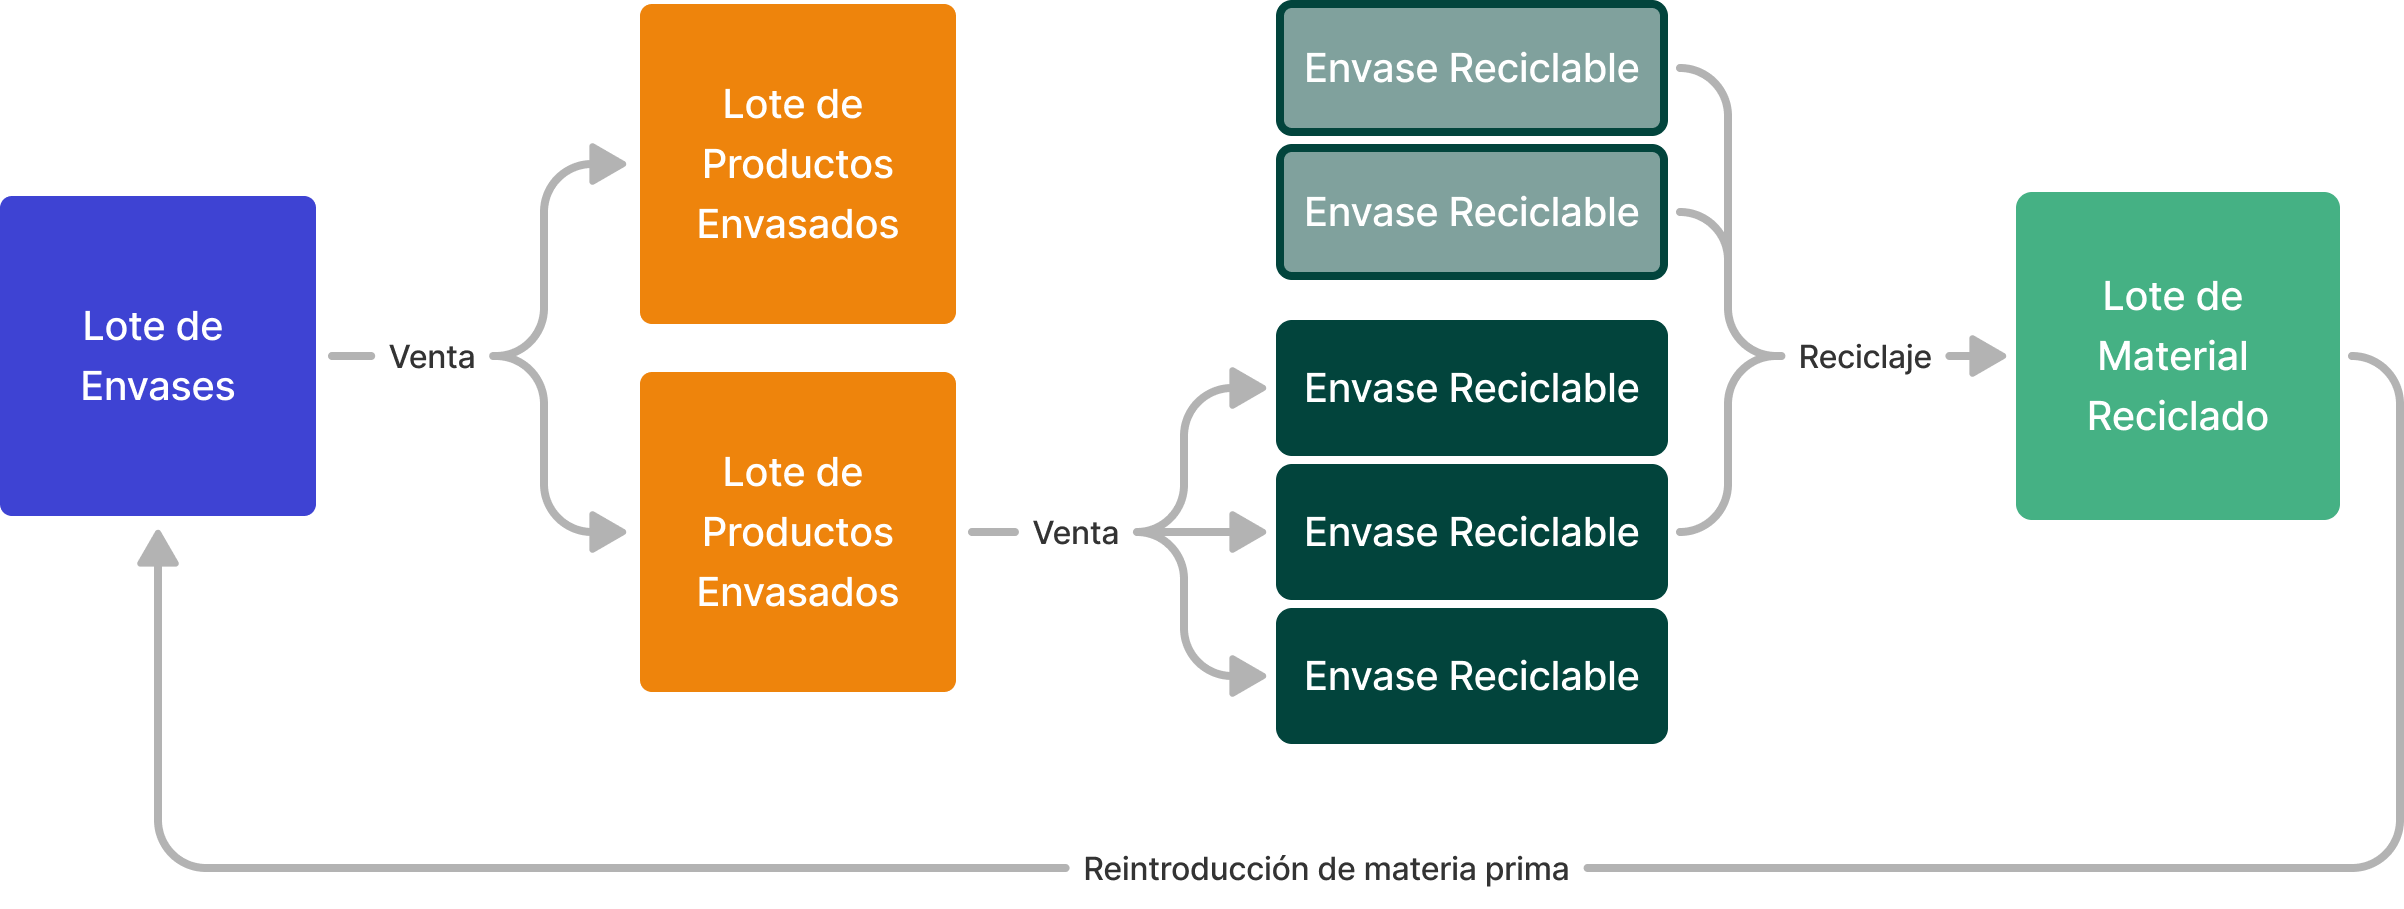
\includegraphics[width=\linewidth]{Figures/data-lifecycle.png}
    \caption{Diagrama de ciclo de vida de los envases de vidrio en el sistema}
    \label{fig:data-lifecycle}
\end{figure}

En primera instancia, se definió la representación de los datos, tanto en la \textit{blockchain} como en la base de datos relacional. Con base en los requerimientos del sistema y la investigación sobre el ciclo de vida del vidrio, se optó por representar cada envase o conjunto de envases con una estructura distinta en cada etapa de su vida útil. Esta decisión se tomó debido a que los envases tienen metadatos, propietarios y agrupaciones diferentes en cada fase del proceso. El flujo de estados de los envases de vidrio, como se observa en la Figura \ref{fig:data-lifecycle}, comienza con un lote de envases producido por el productor primario, que luego se vende a múltiples productores secundarios para crear lotes de productos envasados. Finalmente, los consumidores pueden llevar cada envase vacío a centros de reciclaje, donde se agrupan en lotes de reciclaje para su posterior reprocesamiento. Para mantener la \gls{trazabilidad} completa del ciclo de vida, cada elemento posee una referencia a su ID (identificador) de origen, lo que permite rastrear, a partir de un envase reciclado, el lote original en el que fue producido, su productor y sus metadatos.

\begin{figure}[!b]
    \centering
    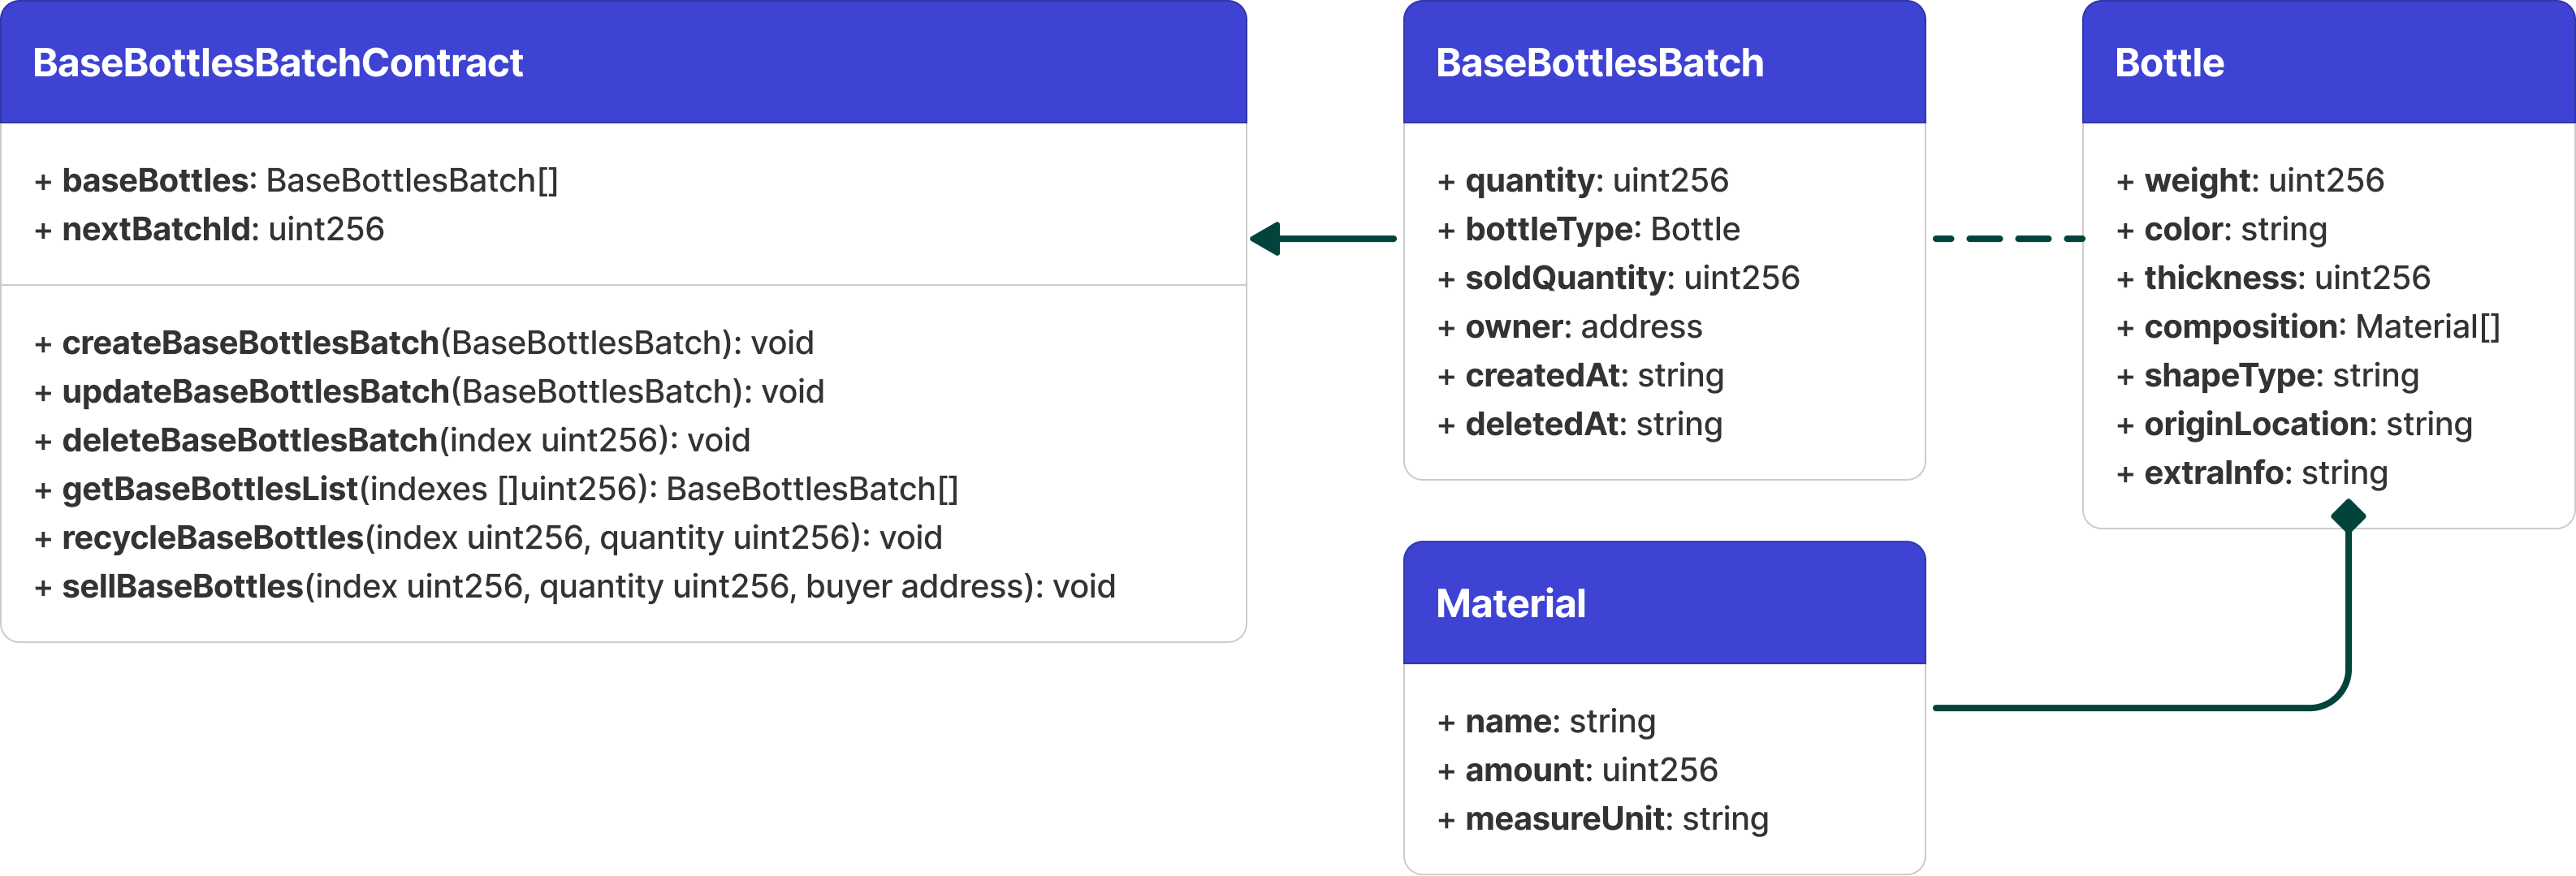
\includegraphics[width=\linewidth]{Figures/uml-producer-contract.png}
    \caption{Diagrama \acrshort{uml} del Contrato de Envases (BaseBottlesBatchContract)}
    \label{fig:bottles-contract-uml}
\end{figure}

A partir de la representación de los datos, se diseñaron los \glspl{contratointeligente} en la \textit{blockchain} para almacenar únicamente la información necesaria para garantizar la trazabilidad de los envases y la integridad de los datos, como un identificador único de cada lote de vidrio, sus metadatos esenciales de producción, el propietario actual y un historial de las transferencias de propiedad y de estado. Al igual que en un sistema de programación orientada a objetos (\gls{oop}), los contratos en Solidity implementan atributos que guardan el estado y métodos que permiten interactuar con él. En lugar de un único contrato monolítico, se decidió implementar tres contratos que interactúan entre sí para lograr mayor modularidad, mantenibilidad y desacoplamiento. A continuación, se detalla la arquitectura de cada uno de ellos, incluyendo sus responsabilidades y la interacción entre ellos. Para cada contrato, se presenta un diagrama de clases \acrshort{uml} (\textit{\acrlong{uml}}) que ilustra su estructura interna, junto con las estructuras de datos relacionadas. Un diagrama de clases \acrshort{uml} es una herramienta visual que se usa en la \gls{ingenieriadesoftware} para modelar la estructura de un sistema orientado a objetos. Describe las clases con sus atributos (datos) y métodos (funciones), y las relaciones entre ellas. Permite visualizar la composición y las interacciones del sistema, facilitando la comunicación y el entendimiento entre los desarrolladores. De forma práctica, actúa como un mapa conceptual que detalla los componentes principales del software antes de su implementación. Dentro del diagrama, los nombres de clases y propiedades se describen en inglés, siguiendo las convenciones de nomenclatura estándar vigentes en programación en entornos profesionales. Posteriormente, en la etapa de codificación, todo el código será implementado en inglés siguiendo este estándar, por lo que se utilizarán los nombres definidos en los diagramas \acrshort{uml} para mantener la coherencia y facilitar la comprensión del código.

\textbf{Contrato de envases: BaseBottlesBatchContract} (Figura \ref{fig:bottles-contract-uml})
 es el punto de partida del ciclo de vida del vidrio, encargado de gestionar la producción inicial de los envases. Sus responsabilidades incluyen registrar lotes de botellas recién fabricadas por el productor primario y sus metadatos (como la cantidad y composición), así como gestionar la transferencia de propiedad a productores secundarios. Sus métodos permiten crear, actualizar y eliminar lotes, además de consultar la información histórica de los mismos. La información de este contrato es consumida por el  contrato \textit{ProductBottlesBatchContract}, proporcionando una referencia al lote original para el siguiente eslabón de la cadena de trazabilidad.

\begin{figure}[!tb]
    \centering
    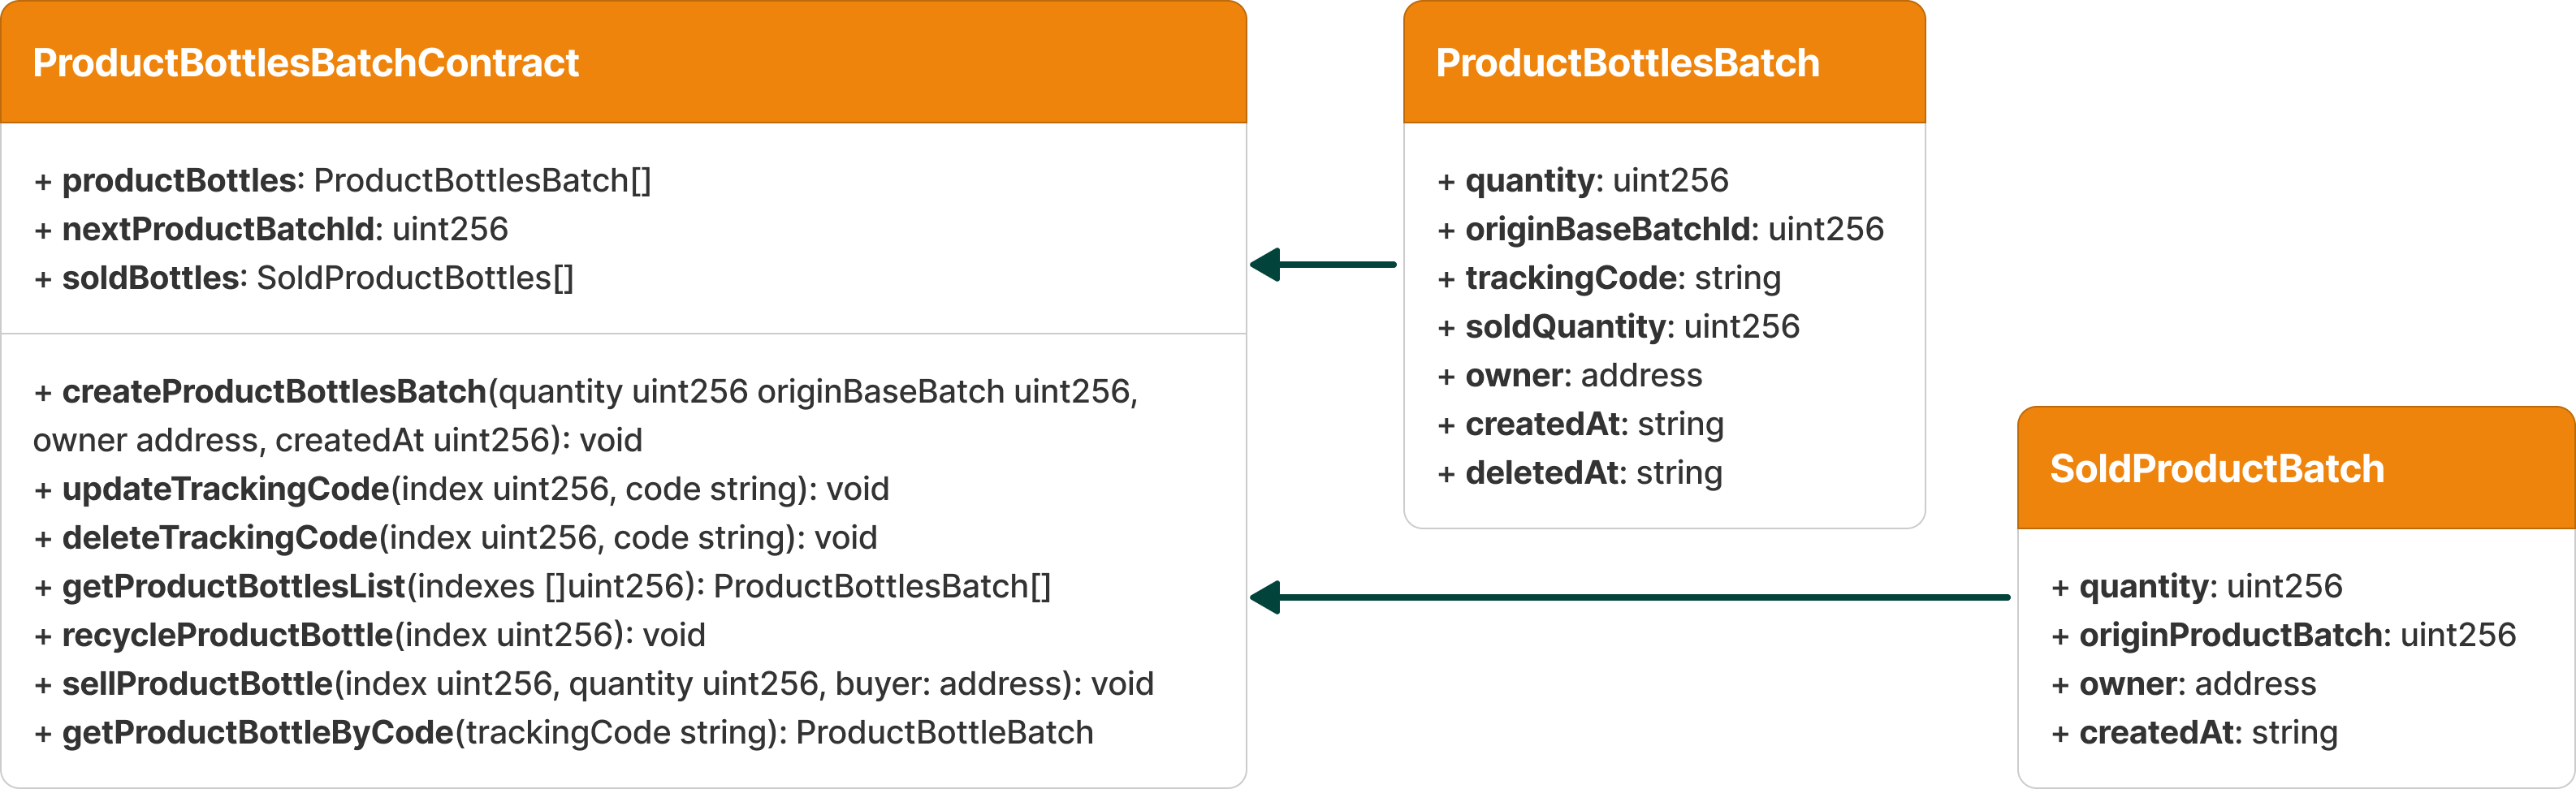
\includegraphics[width=\linewidth]{Figures/uml-product-contract.png}
    \caption{Diagrama \acrshort{uml} del Contrato de Productos (ProductBottlesBatchContract)}
    \label{fig:product-contract-uml}
\end{figure}

\begin{figure}[!b]
    \centering
    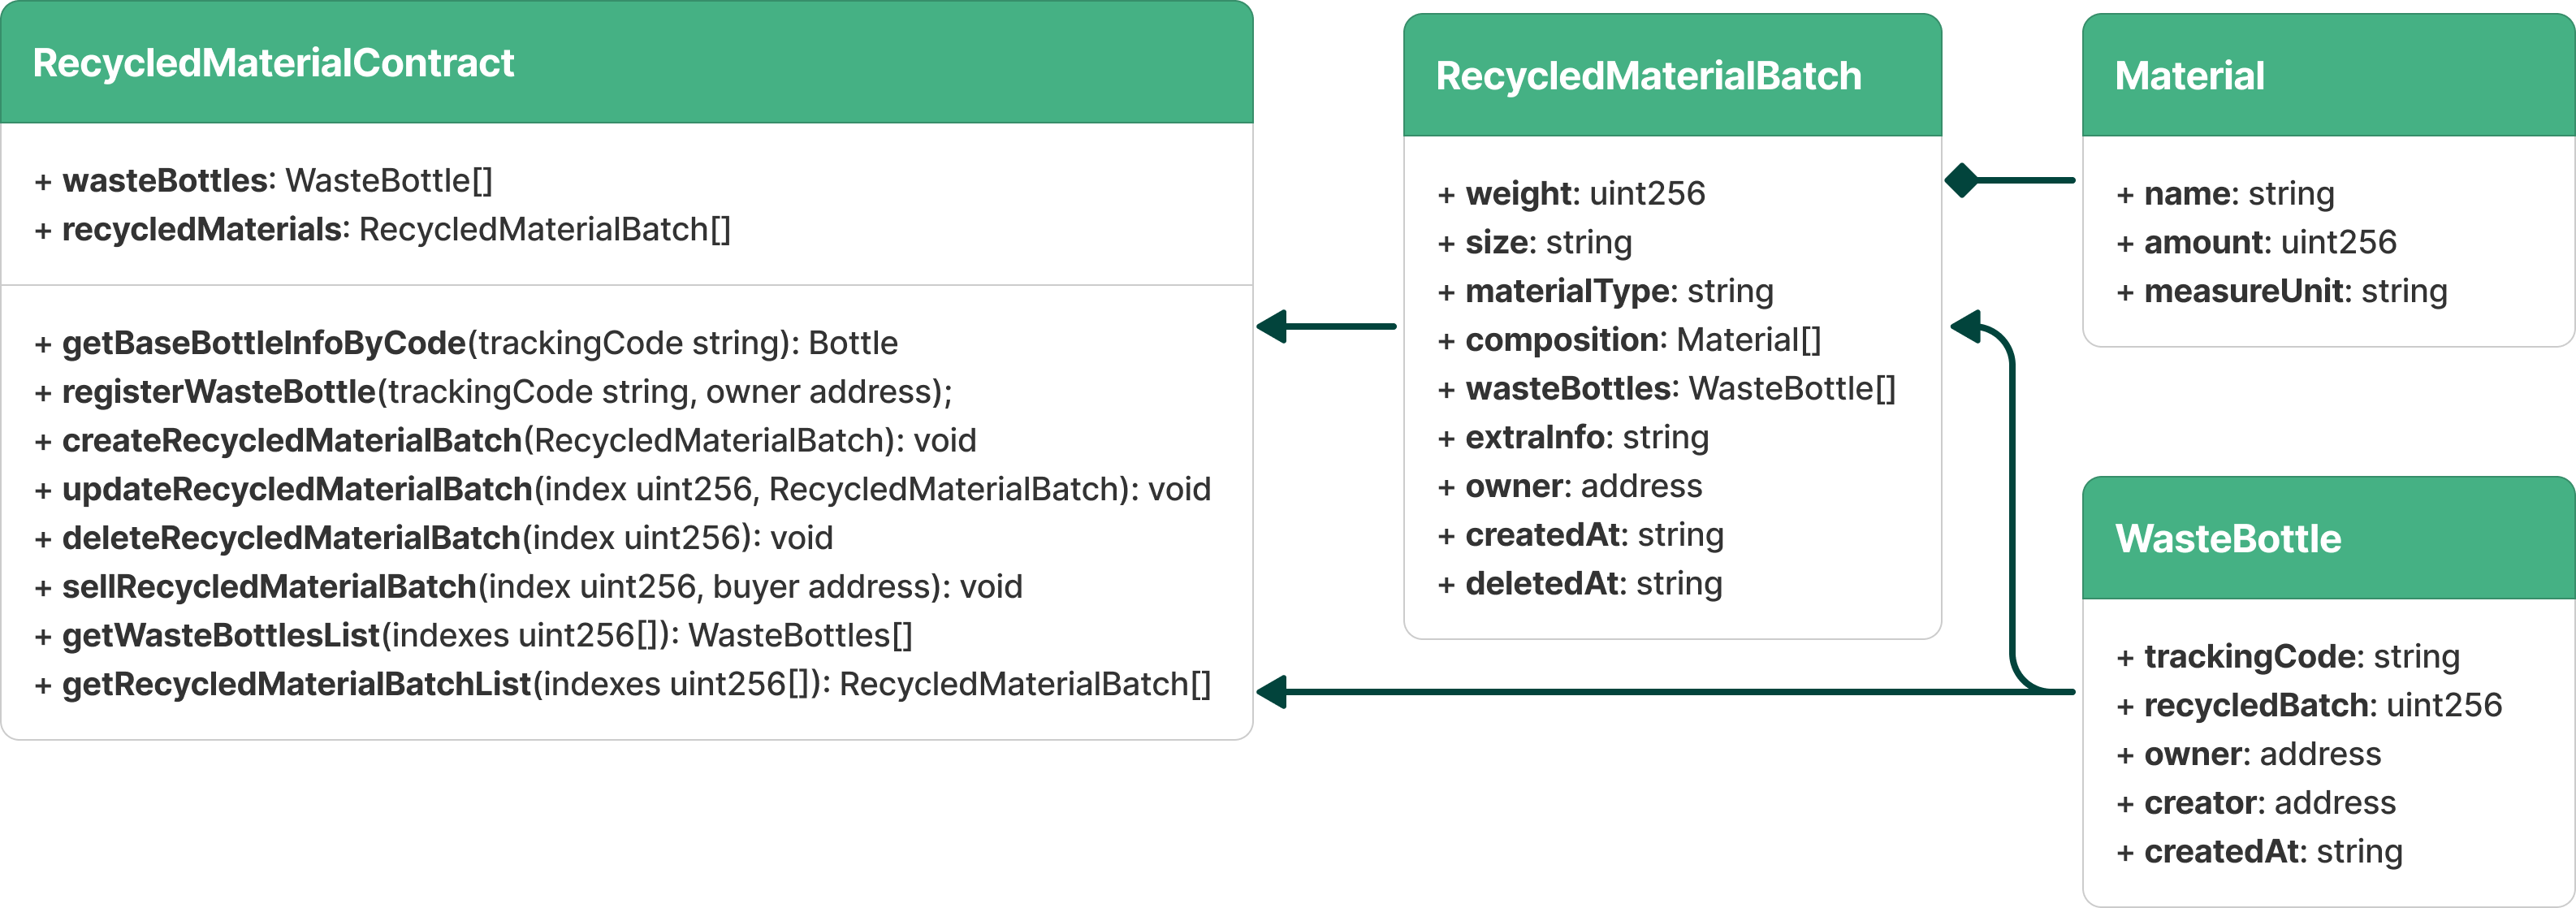
\includegraphics[width=\linewidth]{Figures/uml-recycling-contract.png}
    \caption{Diagrama \acrshort{uml} del Contrato de Reciclaje (RecycleMaterialContract)}
    \label{fig:recycling-contract-uml}
\end{figure}

\textbf{Contrato de productos: ProductBottlesBatchContract} (Figura \ref{fig:product-contract-uml})
 gestiona la segunda fase del ciclo de vida del vidrio, comprende el envasado y la comercialización de estos productos. Este contrato registra los lotes de productos terminados, asociando un código de seguimiento a cada uno y referenciando el lote de envases original del contrato \textit{BaseBottlesBatchContract}. Sus funciones permiten crear lotes de productos, registrar su venta y marcar aquellos envases que se convierten en residuos. La información de seguimiento generada en este contrato juega un rol central en el sistema de trazabilidad, ya que el código de seguimiento introducido en este contrato actúa como el eslabón intermedio que permite vincular el lote de origen de un envase de \textit{BaseBottlesBatchContract} con el envase en \textit{RecycleMaterialContract} cuando el consumidor lo desecha para su posterior reciclaje.

\textbf{Contrato de reciclaje: RecycleMaterialContract} (Figura \ref{fig:recycling-contract-uml})
 cubre la gestión del final de la vida útil de los envases, desde su recolección como residuo hasta su procesamiento como material reciclado. Este contrato almacena los registros de los envases que han sido entregados para reciclaje, permitiendo crear nuevos lotes de material reciclado a partir de ellos. Sus métodos permiten registrar envases de desecho, crear lotes de material reciclado (agrupando envases previamente registrados) y transferir la propiedad de estos lotes a los productores primarios, cerrando de esta forma el ciclo de vida circular del vidrio. La información de seguimiento de los envases provista por el contrato \textit{ProductBottlesBatchContract} es consumida por este contrato, que a su vez genera nuevos lotes de material que pueden ser reutilizados por el contrato \textit{BaseBottlesBatchContract}.

\begin{figure}[!b]
    \centering
    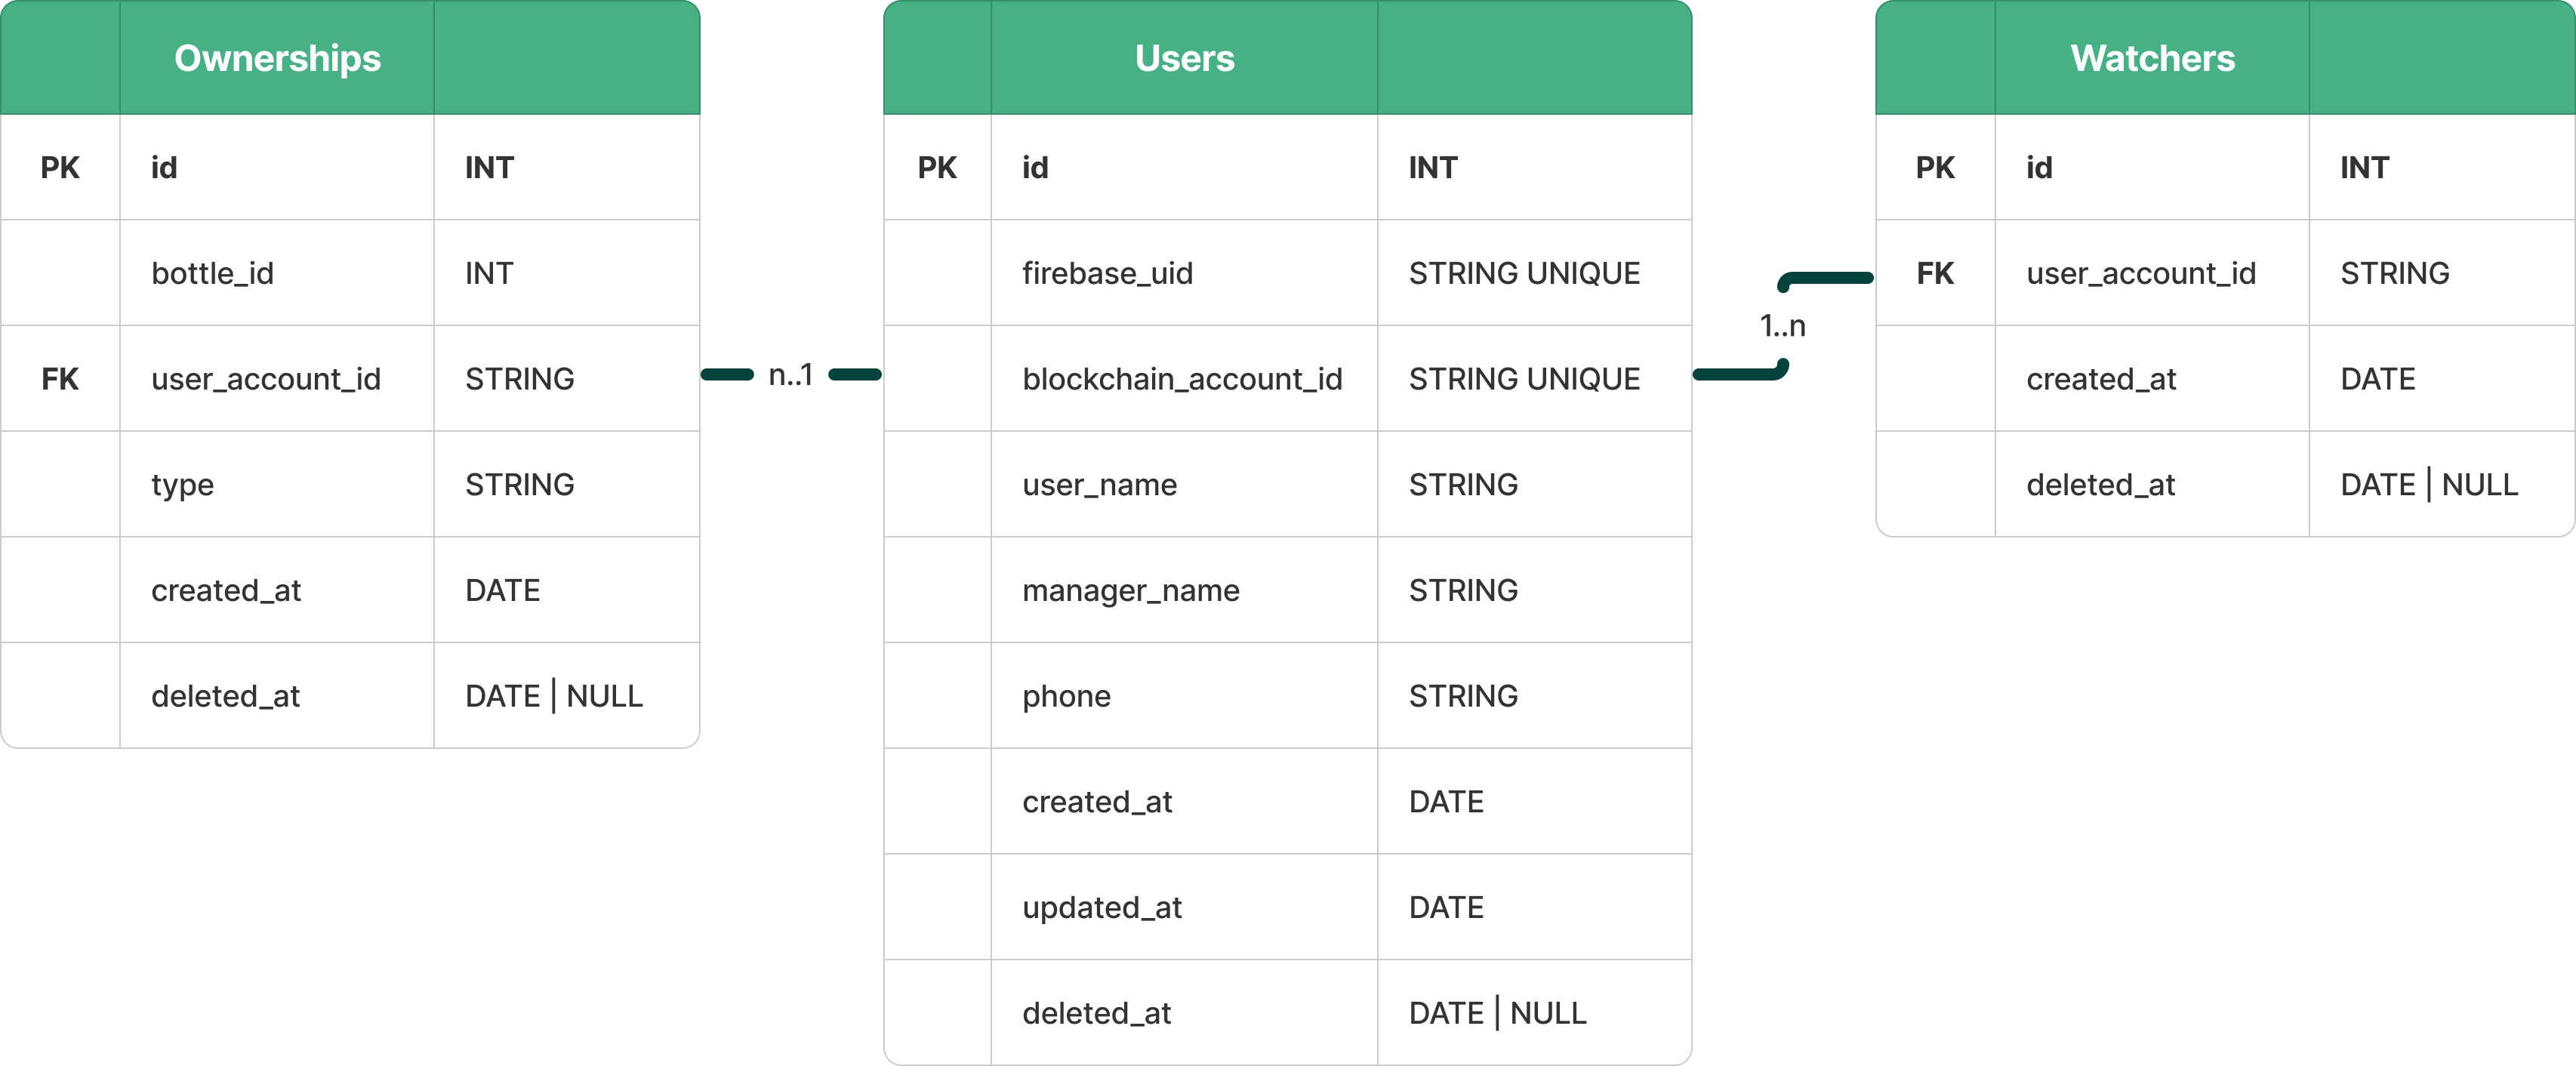
\includegraphics[width=\textwidth]{Figures/db-der.png}
    \caption{Diagrama Entidad-Relación (\gls{der}) del modelo de datos}
    \label{fig:der}
\end{figure}

De forma complementaria a la arquitectura de contratos inteligentes, el diseño de la \gls{basededatos} relacional almacena la información de los usuarios (relacionada con los requerimientos funcionales de autenticación y autorización) y una referencia al ID y propietario de cada lote y envase registrado en la \textit{blockchain}. La relación entre los datos de la \textit{blockchain} y la base de datos relacional se establece mediante el identificador único del lote, que sirve como clave de enlace y permite realizar consultas de metadatos detallados de cada lote. Adicionalmente, en la base de datos relacional se guarda una referencia a cada envase reciclado por los consumidores. Esto permite que cada consumidor pueda acceder al listado de envases que ha reciclado previamente y consultar si efectivamente ha sido procesado, cumpliendo así con el requerimiento funcional asociado (RF-023). En la Figura \ref{fig:der} se presenta un diagrama (DER) que ilustra la relación entre las entidades de la \gls{basededatos}.

\subsection{Arquitectura backend}

En el diseño de arquitectura de la capa \textit{\gls{backend}} se adoptó el patrón \textit{\Gls{cleanarchitecture}} (Arquitectura Limpia) \cite{martin2017clean}, un modelo de diseño que prioriza la separación de las reglas de negocio de las dependencias externas. En este esquema, la implementación de la API se estructura en tres capas principales: \textit{Routers}, \textit{Handlers} y \textit{Repositories}. Los \textit{routers} reciben las solicitudes HTTP y las dirigen a los \textit{handlers} correspondientes, luego los \textit{handlers} contienen la lógica de negocio y orquestan las operaciones, por último, los \textit{repositories} se encargan de la interacción con las fuentes de datos (ya sea la base de datos relacional o la \textit{blockchain}). La comunicación entre estas capas es unidireccional, lo que significa que las capas externas solo pueden acceder a las capas más internas, reforzando así la independencia de la lógica de negocio. La Figura \ref{fig:clean-architecture} ilustra cómo las interfaces externas (como el \textit{frontend} y otros sistemas) interactúan únicamente con los controladores (\textit{routers}), los cuales a su vez interactúan con los casos de uso (\textit{handlers}), que finalmente se comunican con las entidades (\textit{repositories}) para acceder al dominio (datos).

\begin{figure}[!b]
\centering
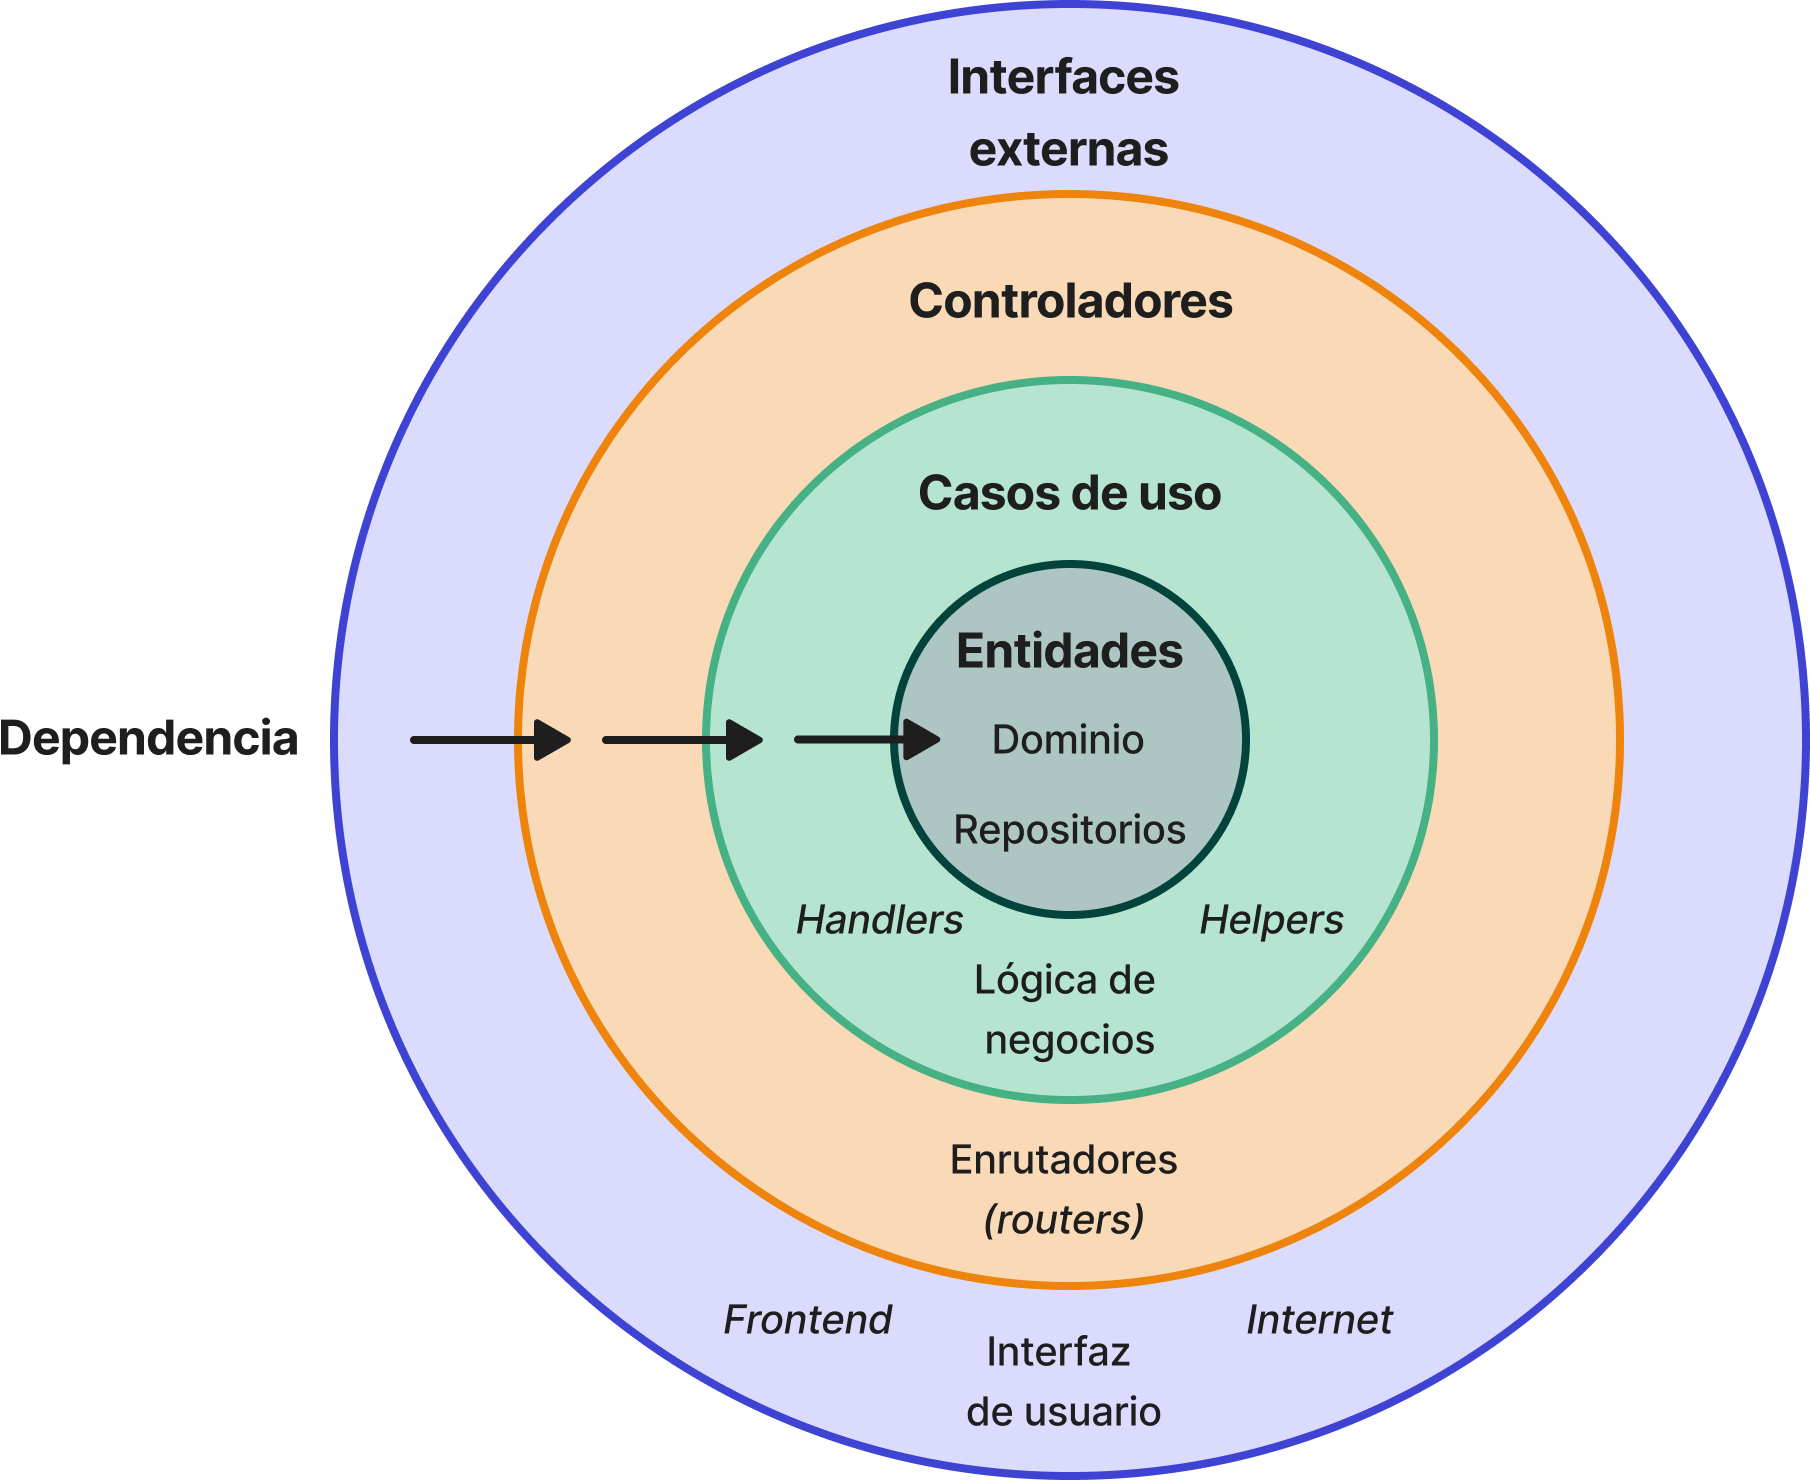
\includegraphics[width=0.6\textwidth]{Figures/clean-architecture.png}
\caption{Modelo \textit{Clean Architecture}}
\label{fig:clean-architecture}
\end{figure}

La elección del patrón \textit{\gls{cleanarchitecture}} se justifica por su capacidad para generar un sistema altamente desacoplado, lo que se traduce en una mayor mantenibilidad del sistema y flexibilidad ante futuros cambios. La lógica de negocio, situada en el núcleo de la arquitectura (\textit{Handlers}), se mantiene independiente de las tecnologías de implementación (infraestructura), la presentación de los datos (\textit{Routers}) y las bases de datos (\textit{Repositories}). Esto es particularmente ventajoso en un sistema de trazabilidad como el planteado en este trabajo, donde la lógica de negocio debe ser estable, pero la interfaz de usuario y las integraciones con otros sistemas (como plataformas de gestión o dispositivos \gls{iot}) pueden evolucionar. A su vez, en este proyecto la arquitectura de la API se ha dividido en módulos de dominio (por ejemplo, gestión de usuarios o trazabilidad de lotes), cada uno de los cuales expone un conjunto de \textit{\glspl{endpoint}} a través de una \gls{apirest}.

En particular, para orquestar la comunicación entre la API, la base de datos relacional y la \textit{blockchain}, se implementó un patrón de repositorios que unifica las operaciones de lectura y escritura. De esta forma, el \textit{handler} puede manejar todos los datos de manera uniforme, sin importar si el repositorio los obtuvo de la \textit{blockchain} o de la base de datos relacional, ya que esta lógica de acceso a datos se abstrae en el repositorio. Por ejemplo, al registrar un nuevo lote, el \textit{handler} valida la información y luego instruye al repositorio de la \textit{blockchain} para registrar la transacción y al repositorio de la base de datos relacional para almacenar la referencia del lote. En este caso, el patrón de diseño \textit{Clean Architecture} permite abstraer la complejidad de la arquitectura híbrida, proporcionando una interfaz de programación unificada a la capa de lógica de negocio.

\subsection{Arquitectura frontend}

La interfaz de usuario del sistema se diseñó como una aplicación web, con el objetivo de proporcionar una experiencia de usuario fluida, accesible desde cualquier dispositivo con conexión a Internet y sin necesidad de instalar software adicional. Debido al alcance limitado del trabajo, se decidió implementar una interfaz diseñada para computadoras de escritorio, dado que es el caso de uso más frecuente en sistemas de gestión y trazabilidad. La aplicación podrá accederse en dispositivos móviles, pero no se ha priorizado la implementación adaptada para estos dispositivos, por lo que la interfaz puede resultar menos amigable en pantallas pequeñas. La interfaz se estructuró mediante una arquitectura basada en componentes, un patrón de diseño que promueve la creación de elementos reutilizables, modulares e independientes, que es el patrón recomendado por librerías como React y \textit{frameworks} como Next.js.

\begin{figure}[!t]
\centering
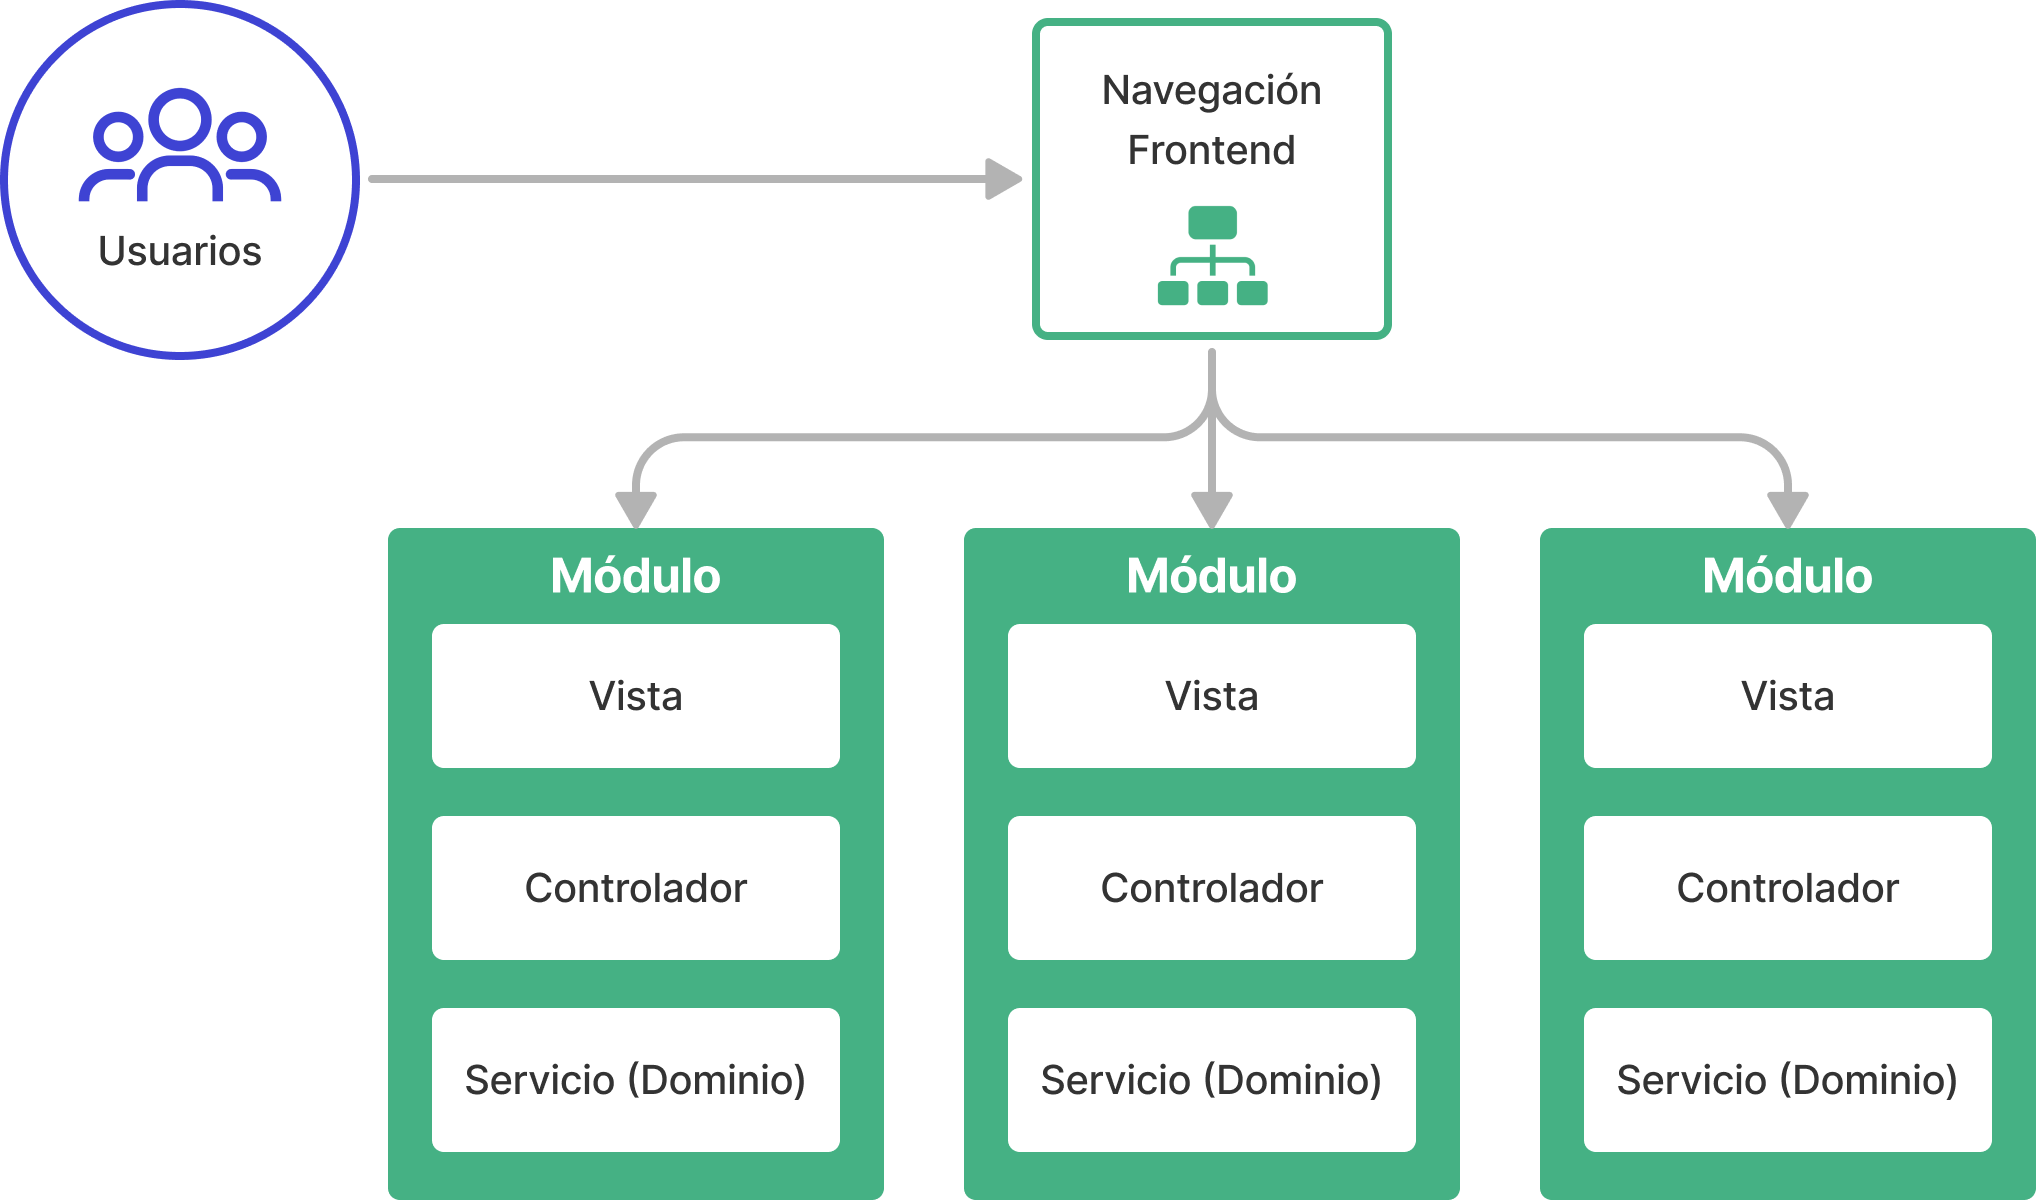
\includegraphics[width=0.8\textwidth]{Figures/frontend-architecture.png}
\caption{Arquitectura de módulos \textit{\gls{frontend}}}
\label{fig:frontend-architecture}
\end{figure}

Para la estructuración interna del código, se eligió implementar una arquitectura Modelo Vista-Controlador (\gls{mvc}), que establece una clara separación de responsabilidades: la vista implementa la interfaz de usuario, el controlador maneja la lógica y las interacciones, y el modelo (en este caso, un servicio) se comunica con el \textit{\gls{backend}}. Esta metodología, combinada con la arquitectura de componentes, facilita una construcción rápida y consistente de cada vista, al mismo tiempo que mejora la mantenibilidad del código a largo plazo, ya que cada componente puede ser actualizado sin afectar otras partes del sistema. En la Figura \ref{fig:frontend-architecture} se ilustra la arquitectura de componentes y módulos del \textit{frontend}, donde los usuarios navegan por las distintas vistas de la aplicación y cada una está compuesta por un módulo con un componente de vista, un controlador que implementa la lógica y un servicio que actúa como modelo, el cual se encarga de enviar solicitudes a la \gls{api} \textit{backend} para interactuar con los datos.

\begin{figure}[!b]
    \centering
    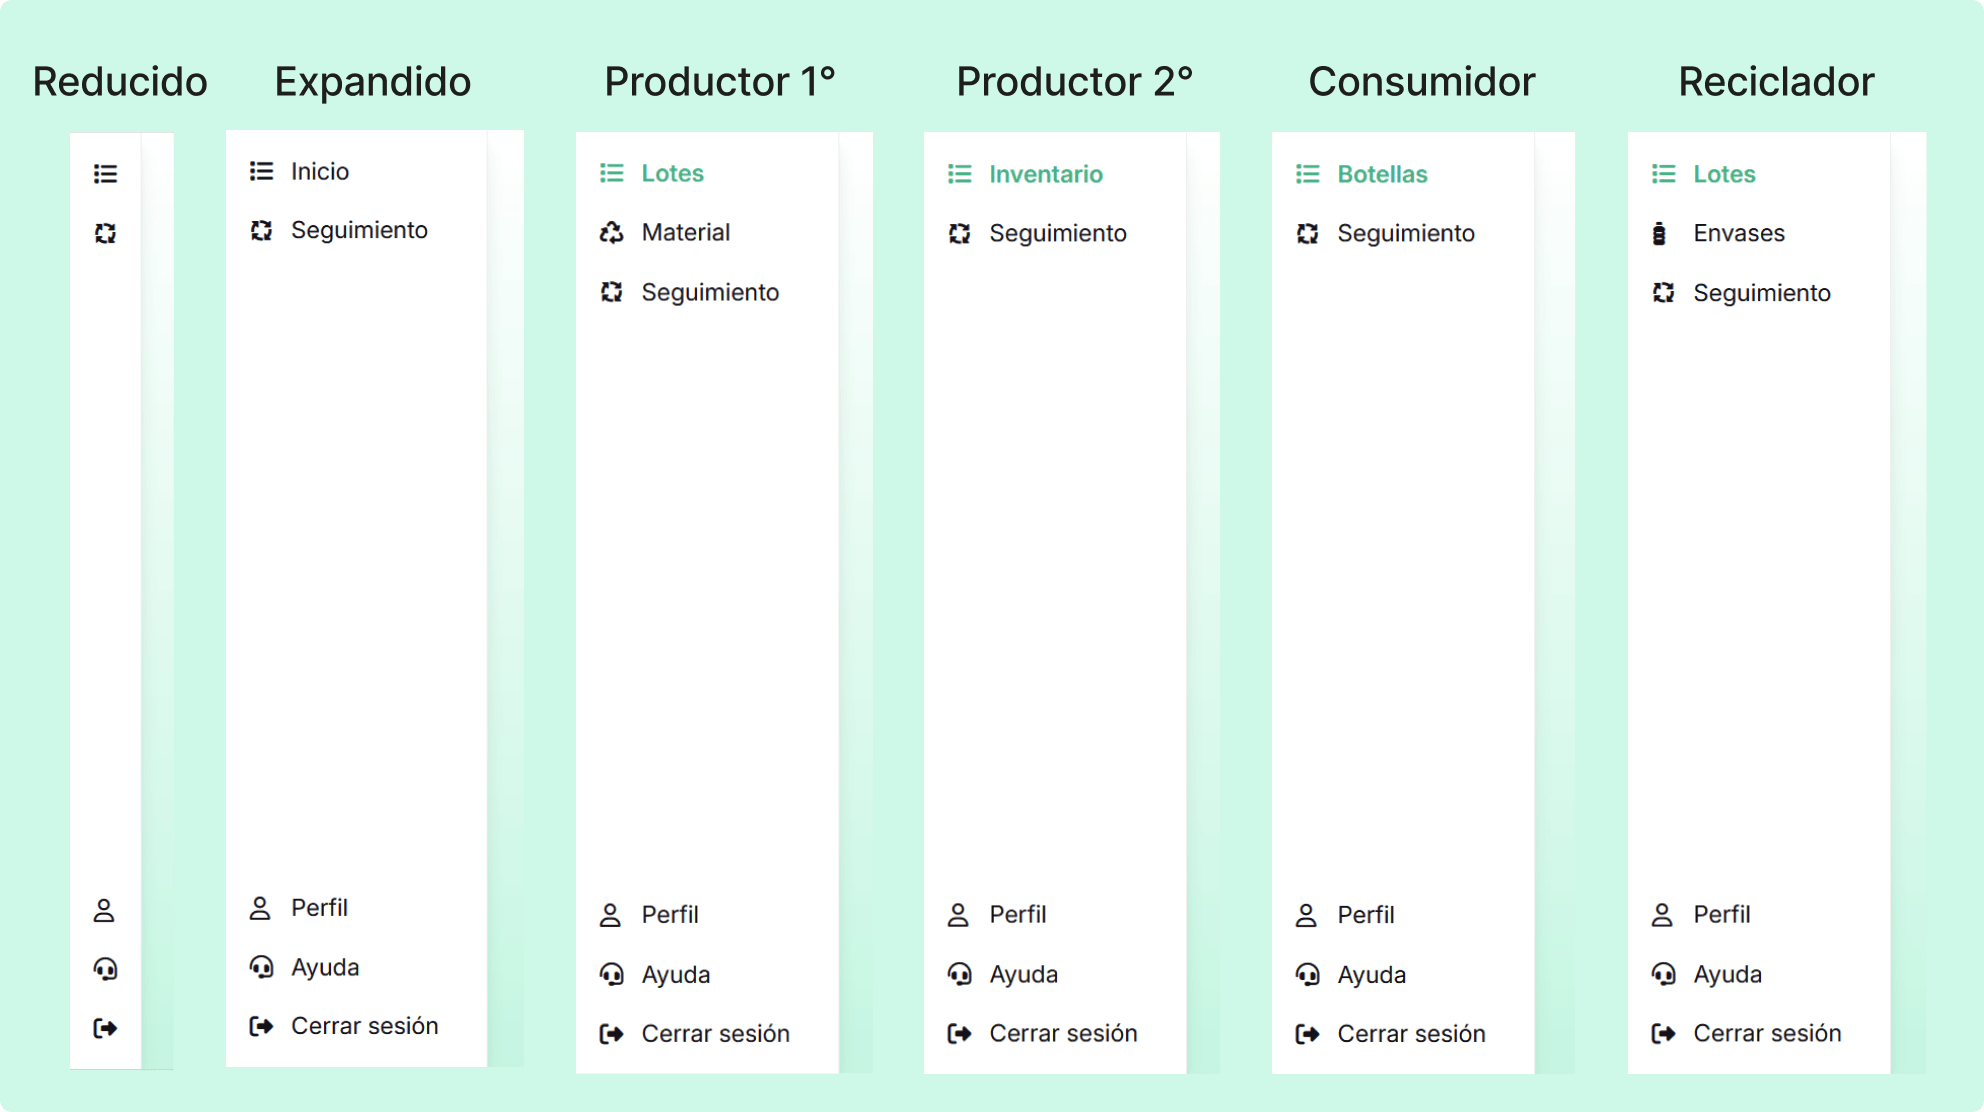
\includegraphics[width=\textwidth]{Figures/frontend-navigation.png}
    \caption{Diseño de casos de la barra lateral de navegación de la aplicación para cada rol}
    \label{fig:frontend-navigation}
\end{figure}

La estructura de la interfaz de usuario se organizó en módulos funcionales por cada rol de usuario, lo cual se alinea con la división de responsabilidades del diseño de arquitectura de \textit{backend} y capa de datos. Por ejemplo, se definieron vistas específicas para el registro y la gestión de lotes por parte de los productores, junto con una interfaz de consulta para los consumidores. En la Figura \ref{fig:frontend-navigation} se puede observar el diseño de la navegación de la aplicación, que consiste en una barra lateral comprimida que se expande al posicionar el cursor sobre ella, mostrando accesos directos a las pantallas disponibles según el rol del usuario autenticado. El contenido de la barra lateral varía dinámicamente según el rol del usuario autenticado para permitir un acceso rápido a las funcionalidades relevantes para cada tipo de usuario. En el Apéndice \ref{cp:user-flows} se encuentran documentados los flujos de usuario para cada rol con imágenes de sus respectivas pantallas y las acciones que conectan el flujo.

\begin{figure}[!t]
    \centering
    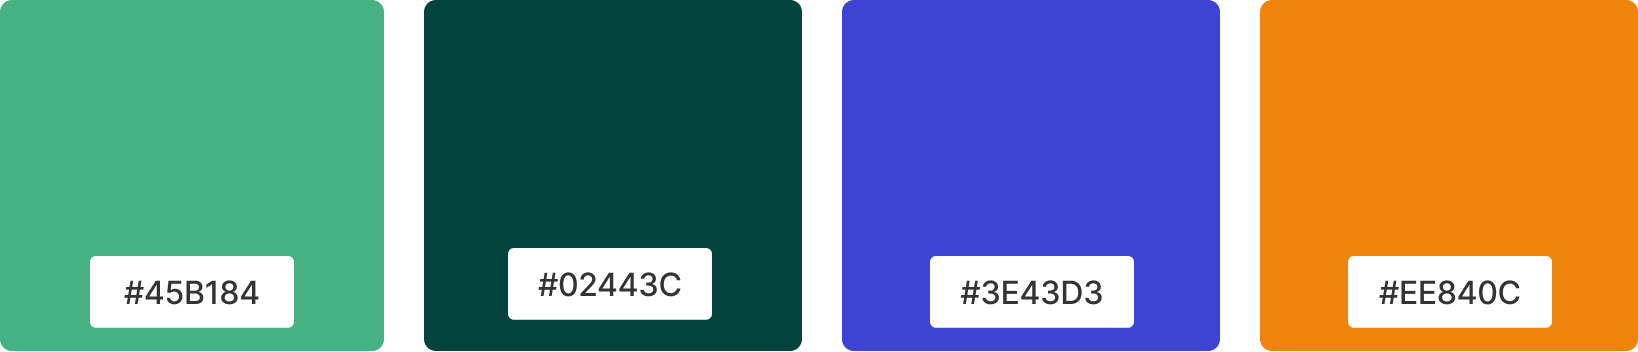
\includegraphics[width=0.8\textwidth]{Figures/frontend-palette.png}
    \caption{Identidad de marca de la aplicación}
    \label{fig:frontend-brand}
\end{figure}

Por otro lado, para asegurar una identidad visual consistente en la aplicación, se definió un sistema de diseño con una paleta de colores basada en tonalidades de verde con el objetivo de transmitir el compromiso ambiental del proyecto mediante la economía circular, así como también tipografías e iconografía que complementan esta estética. En la Figura \ref{fig:frontend-brand} se puede observar una muestra de la identidad de marca de la aplicación, a través de su paleta de colores, que posee un color primario (verde), un color secundario (verde oscuro) y colores complementarios (azul y anaranjado) para resaltar elementos importantes en la interfaz.

Con la definición de las especificaciones detalladas de la arquitectura de componentes para el \textit{frontend}, el \textit{backend} y la capa de datos, el proceso de desarrollo posterior puede ser más fluido, organizado y predecible. En el siguiente capítulo se abordará el proceso de implementación del prototipo tecnológico, a través del cual se materializarán los diseños aquí descritos en un software funcional que cumpla con los requerimientos establecidos.
